\documentclass{article}

\usepackage{etoolbox}
\newtoggle{arxiv}
\toggletrue{arxiv}




\iftoggle{arxiv}{}{
\PassOptionsToPackage{numbers,sort,compress}{natbib}
\usepackage{neurips_2024}
}







\usepackage[utf8]{inputenc} %
\usepackage[T1]{fontenc}    %
\usepackage{hyperref}       %
\usepackage{url}            %
\usepackage{booktabs}       %
\usepackage{amsfonts}       %
\usepackage{nicefrac}       %
\usepackage{microtype}      %
\usepackage{xcolor}         %
\usepackage{amsmath,amsthm,amssymb}

\usepackage{algorithm}
\usepackage{algorithmic}

\usepackage{caption}
\captionsetup[figure]{font=small}
\usepackage{subcaption}
\usepackage{multirow}

\usepackage{xspace}
\usepackage{wrapfig}

\usepackage{pifont}
\newcommand{\xmark}{\ding{55}}

\usepackage[capitalise]{cleveref}  %

\crefname{section}{\S\hspace{-0.2em}}{\S\S\hspace{-0.2em}}
\crefname{subsection}{\S\hspace{-0.2em}}{\S\S\hspace{-0.2em}}
\crefname{subsubsection}{\S\hspace{-0.2em}}{\S\S\hspace{-0.2em}}

\usepackage{comment}
\usepackage[inline]{enumitem}

\usepackage{graphicx}
\usepackage{grffile}
\usepackage{color}

\usepackage{newtxmath}

\iftoggle{arxiv}{
\usepackage[numbers,sort]{natbib}
}{}

\usepackage{import}

\usepackage{tikz-cd}
\usepackage{tikz}

\providecommand{\main}{.}

\newtoggle{todo}
\toggletrue{todo}
\newcommand{\todo}[1]{\iftoggle{todo}{\textcolor{cyan}{[TODO: #1]}}{}}

\newtoggle{comment}
\togglefalse{comment} %
\newcommand{\TD}[1]{\iftoggle{comment}{\textcolor{magenta}{[TD: #1]}}{}}


\renewcommand{\max}{\mathrm{max}}
\renewcommand{\exp}{\mathrm{exp}}
\newcommand{\abs}[1]{\left\lvert#1\right\rvert}
\newcommand{\norm}[1]{\left\|{#1}\right\|} %
\newcommand{\diag}{\mathrm{diag}}
\newcommand{\softmax}{\mathrm{softmax}}
\newcommand{\rowmax}{\mathrm{rowmax}}
\newcommand{\rowsum}{\mathrm{rowsum}}
\newcommand{\dsoftmax}{\mathrm{dsoftmax}}
\providecommand{\tr}{\mathop{\rm tr}}

\newcommand{\defeq}{:=}

\newcommand{\RR}{\mathbb{R}}

\newcommand{\vQ}{\mathbf{Q}}
\newcommand{\vK}{\mathbf{K}}
\newcommand{\vV}{\mathbf{V}}
\newcommand{\vdQ}{\mathbf{dQ}}
\newcommand{\vdK}{\mathbf{dK}}
\newcommand{\vdV}{\mathbf{dV}}
\newcommand{\vS}{\mathbf{S}}
\newcommand{\vdS}{\mathbf{dS}}
\newcommand{\vP}{\mathbf{P}}
\newcommand{\vdP}{\mathbf{dP}}
\newcommand{\vU}{\mathbf{U}}
\newcommand{\vW}{\mathbf{W}}
\newcommand{\vT}{\mathbf{T}}
\newcommand{\vX}{\mathbf{X}}
\newcommand{\vO}{\mathbf{O}}
\newcommand{\vdO}{\mathbf{dO}}
\newcommand{\vM}{\mathbf{M}}
\newcommand{\vZ}{\mathbf{Z}}

\newcommand{\fa}{\textsc{FlashAttention}\xspace}
\newcommand{\sysnameone}{\textsc{FlashAttention}\xspace}
\newcommand{\faa}{\textsc{FlashAttention-2}\xspace}
\newcommand{\fat}{\textsc{FlashAttention-3}\xspace}  %

\newtheorem{theorem}{Theorem}
\newtheorem*{theorem*}{Theorem}
\newtheorem{corollary}[theorem]{Corollary}
\newtheorem{definition}{Definition}
\newtheorem{lemma}[theorem]{Lemma}
\newtheorem{claim}[theorem]{claim}
\newtheorem{example}{Example}
\newtheorem{proposition}[theorem]{Proposition}


\newcommand*\samethanks[1][\value{footnote}]{\footnotemark[#1]}
\usepackage{authblk}
\makeatletter
\renewcommand\AB@affilsepx{ \protect\Affilfont}
\makeatother

\iftoggle{arxiv}{
  \setlength{\textwidth}{6.9in}
  \setlength{\textheight}{9in}
  \setlength{\oddsidemargin}{0in}
  \setlength{\evensidemargin}{0in}
  \setlength{\topmargin}{-0.5in}
  \newlength{\defbaselineskip}
  \setlength{\defbaselineskip}{\baselineskip}
  \setlength{\marginparwidth}{0.8in}
}{
\usepackage[compact]{titlesec}
\titlespacing{\section}{0pt}{*1}{*0}
\titlespacing{\subsection}{0pt}{*1.5}{*0}

\usepackage[subtle, mathdisplays=normal, charwidths=normal, leading=normal]{savetrees}

\addtolength\textfloatsep{-0.5em}
\addtolength\intextsep{-0.2em}


\def\setstretch#1{\renewcommand{\baselinestretch}{#1}}
\setstretch{0.985}
\addtolength{\parskip}{-1pt}

}

\title{FlashAttention-3:\\ Fast and Accurate Attention with Asynchrony and Low-precision}

\iftoggle{arxiv}{
  \author[$^1$]{Jay Shah\thanks{Equal contribution}}
  \author[$^1$]{Ganesh Bikshandi\samethanks}
  \author[$^2$]{Ying Zhang}
  \author[$^{3,4}$]{Vijay Thakkar}
  \author[$^3$]{Pradeep Ramani}
  \author[$^{5,6}$]{Tri Dao}
  \affil[$^1$]{Colfax Research}
  \affil[$^2$]{Meta}
  \affil[$^3$]{NVIDIA}
  \affil[$^4$]{Georgia Tech}
  \affil[$^5$]{Princeton University}
  \affil[$^6$]{Together AI\newline}
  \affil[ ]{\hspace{-2em}{\small\texttt{\{jayhshah,ganesh\}@colfax-intl.com},
      \texttt{yingz@meta.com}, \texttt{\{vithakkar,prraman\}@nvidia.com}, \texttt{tri@tridao.me}}}
}{



\author{%
  Jay Shah\thanks{Equal contribution}\: $^{1}$,
  Ganesh Bikshandi\samethanks\: $^{1}$, Ying Zhang $^{2}$, Vijay Thakkar $^{3,4}$,
  Pradeep Ramani $^{3}$, Tri Dao$^{8,9}$\\
  $^1$ Colfax Research\\
  $^2$ Meta\\
  $^3$ NVIDIA \\
  $^4$ Georgia Institute of Technology\\
  $^8$ Princeton University\\
  $^9$ Together AI\\
  {\small\texttt{\{tri\}@tridao.me}}
}
}

\begin{document}


\maketitle


\begin{abstract}
\begin{abstract}
There is a widely-spread claim that GANs are difficult to train, and GAN architectures in the literature are littered with empirical tricks. We provide evidence against this claim and build a modern GAN baseline in a more principled manner. First, we derive a well-behaved regularized relativistic GAN loss that addresses issues of mode dropping and non-convergence that were previously tackled via a bag of ad-hoc tricks. We analyze our loss mathematically and prove that it admits local convergence guarantees, unlike most existing relativistic losses. Second, this loss allows us to discard all ad-hoc tricks and replace outdated backbones used in common GANs with modern architectures. Using StyleGAN2 as an example, we present a roadmap of simplification and modernization that results in a new minimalist baseline---\modelName (``Re-GAN''). Despite being simple, our approach surpasses StyleGAN2 on FFHQ, ImageNet, CIFAR, and Stacked MNIST datasets, and compares favorably against state-of-the-art GANs and diffusion models.\\
Code: \href{https://www.github.com/brownvc/R3GAN}{https://www.github.com/brownvc/R3GAN}
\end{abstract}
\end{abstract}


\section{Introduction}
\label{sec:intro}


Transformers, in particular decoder-only models (e.g.\ GPT~\citep{brown2020language}, Llama~\citep{touvron2023llama}) which process input sequences in a causal fashion, are one of the main drivers of modern deep learning's success.
Numerous approaches attempt to approximate the core attention layer to address its efficiency issues~\citep{tay2022efficient}, such as scaling quadratically in sequence length during training and requiring a cache of size linear in sequence length during autoregressive generation.
In parallel, a class of alternative sequence models, structured state-space models (SSMs), have emerged with linear scaling in sequence length during training and constant state size during generation.
They show strong performance on long-range tasks (e.g. S4~\citep{gu2022efficiently}) and recently matched or beat Transformers on language modeling (e.g. Mamba \citep{gu2023mamba}) at small to moderate scale.
However, the development of SSMs have appeared disjoint from the community's collective effort to improve Transformers, such as understanding them theoretically as well as optimizing them on modern hardware.
As a result, it is more difficult to understand and experiment with SSMs compared to Transformers, and it remains challenging to train SSMs as efficiently as Transformers from both an algorithmic and systems perspective.


Our main goal is to develop a rich body of theoretical connections between structured SSMs and variants of attention.
This will allow us to transfer algorithmic and systems optimizations originally developed for Transformers to SSMs, towards the goal of building foundation models that perform better than Transformers while scaling more efficiently in sequence length.
A milestone contribution in this direction was the \textbf{Linear Attention (LA)} framework \citep{katharopoulos2020transformers},
which derived a connection between autoregressive attention and linear RNNs
by showing the equivalence between ``dual forms'' of quadratic kernelized attention and a particular linear recurrence.
This duality allows new capabilities such as the ability to have both efficient parallelizable training and efficient autoregressive inference.
In the same spirit, this paper provides multiple viewpoints connecting linear-complexity SSMs with quadratic-complexity forms to combine the strengths of SSMs and attention.%
\footnote{Technically speaking, these connections only relate to certain flavors of attention; the title of this paper is an homage to \citet{katharopoulos2020transformers} which first showed that ``Transformers are RNNs''.}

\iftoggle{arxiv}{
\begin{wrapfigure}{R}{0.48\linewidth}
  \begin{center}
    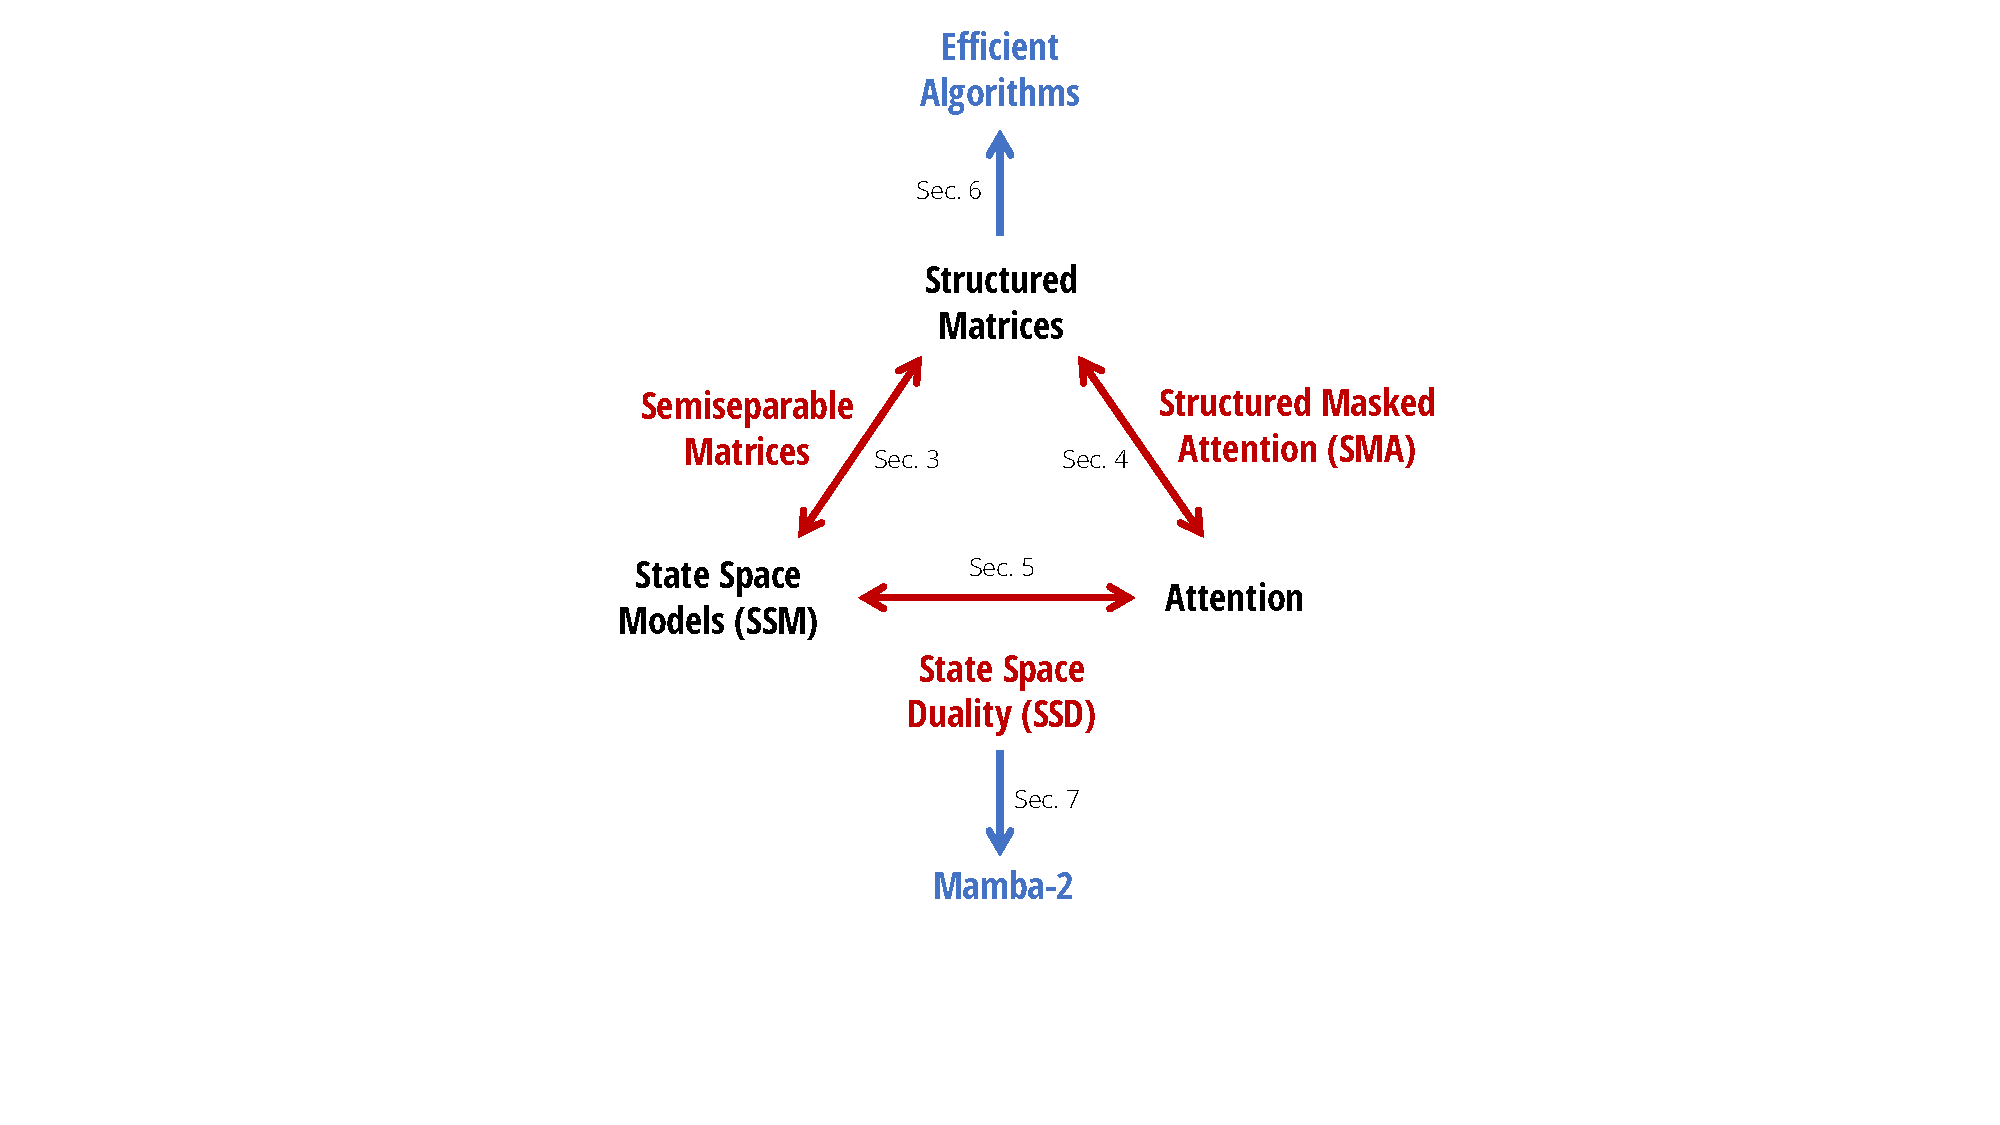
\includegraphics[width=\linewidth]{fig/ssd_roadmap.pdf}
  \end{center}
  \caption{
    (\textbf{Structured State-Space Duality}.)
    This paper fleshes out the relationship between state space models and attention through the bridge of structured matrices.
  }
  \label{fig:roadmap}
\end{wrapfigure}
}{}

\para{State Space Duality.}
Our framework connecting structured SSMs and variants of attention, which we call \textbf{structured state space duality} (SSD),
is made through the abstractions of \textbf{structured matrices}:
matrices with subquadratic parameters and multiplication complexity.
We develop two broad frameworks for representing sequence models, one as matrix transformations and one as tensor contractions, which each reveal different perspectives of the duality.
Our technical contributions include:
\begin{itemize}[leftmargin=*,itemsep=0pt,topsep=0pt]
  \item We show an equivalence between state space models and a well-studied family of structured matrices called \textbf{semiseparable matrices}\iftoggle{arxiv}{ (\cref{sec:ssm})}{}.
    This connection is at the heart our framework, revealing new properties and algorithms for SSMs. A central message of this paper is that \emph{different methods of computing state space models can be reframed as various matrix multiplication algorithms on structured matrices}.
  \item We significantly improve the theory of linear attention~\citep{katharopoulos2020transformers}.
    We first provide an incisive proof of its recurrent form through the language of tensor contractions, and then generalize it to a new family of \textbf{structured masked attention (SMA)}\iftoggle{arxiv}{ (\cref{sec:attention})}{}.
  \item We connect SSMs and SMA, showing that they have a large intersection that are duals of each other, possessing both SSM-like linear and attention-like quadratic forms\iftoggle{arxiv}{ (\cref{sec:ssd})}{}.
    \iftoggle{arxiv}{We also prove that any kernel attention method possessing a fast recurrent form must be an SSM.}{}
\end{itemize}


Beyond its intrinsic theoretical value, our framework opens up a broad set of directions for understanding and improving sequence models.

\para{Efficient Algorithms.}
First and most importantly, our framework exposes new efficient and easily-implementable algorithms for computing SSMs\iftoggle{arxiv}{ (\cref{sec:efficient})}{}.
We introduce a new \textbf{SSD algorithm}, based on block decompositions of semiseparable matrices, that takes advantage of both the linear SSM recurrence and quadratic dual form, obtaining optimal tradeoffs on all main efficiency axes (e.g. training and inference compute, memory usage, and ability to leverage matrix multiplication units on modern hardware).
A dedicated implementation of SSD is $2-8\times$ faster than the optimized selective scan implementation of Mamba, while simultaneously allowing for much larger recurrent state sizes ($8\times$ the size of Mamba or even higher, with minimal slowdown).
SSD is highly competitive with optimized implementations of softmax attention (FlashAttention-2~\citep{dao2023flashattention2}), crossing over at sequence length 2K and 6$\times$ faster at sequence length 16K.


\iftoggle{arxiv}{
\para{Architecture Design.}
One major obstacle to adopting new architectures such as SSMs is the ecosystem tailored to Transformers, such as hardware-efficient optimization and parallelism techniques for large-scale training.
Our framework allows using established conventions and techniques for attention to build a vocabulary of architecture design choices for SSMs, and further improve them (\cref{sec:architecture}).
For example, we introduce the analog of heads from multi-head attention (MHA) to SSMs.
We show that the Mamba architecture is a \textbf{multi-input SSM (MIS)} that turns out to be analogous to \textbf{multi-value attention (MVA)}, and compare other variants of Mamba with different head structures.

We also use these ideas to make slight modifications to the Mamba block, which allows tensor parallelism to be implemented (e.g. in the style of Megatron~\citep{shoeybi2019megatron}).
The main ideas include introducing grouped-value attention (GVA) head structure, and moving all data-dependent projections to occur in parallel at the beginning of the block.


}{
  \para{Mamba-2.}
  Additionally, inspired by the connection between SSMs and Transformers, we slightly modify the neural network architecture of Mamba by moving all data-dependent projections to occur in parallel at the beginning of the block. %
}
The combination of the modified parallel Mamba block, together with using SSD as the inner SSM layer, results in the \textbf{Mamba-2} architecture.
We investigate Chinchilla scaling laws for Mamba-2 in the same setting as Mamba, finding that it Pareto dominates Mamba and Transformer++ in both perplexity and wall-clock time.
We additionally train a family of Mamba-2 models at varying sizes on the Pile, showing that it matches or outperforms Mamba and open source Transformers on standard downstream evaluations.
For example, Mamba-2 with 2.7B parameters trained on 300B tokens on the Pile outperforms Mamba-2.8B, Pythia-2.8B and even Pythia-6.9B trained on the same dataset.

\iftoggle{arxiv}{
\paragraph{Systems Optimizations.}
The SSD framework connects SSMs and Transformers, allowing us to leverage a rich body of work on systems optimizations developed for Transformers~(\cref{sec:systems}).
\begin{itemize}[leftmargin=*,itemsep=0pt,topsep=0pt]
  \item For example, Tensor Parallelism (TP) is an important model parallelism technique to train large Transformer models by splitting each layer across GPUs on the same node.
    We design Mamba-2 to be TP-friendly, reducing the number of synchronization point per block by half.
  \item For very long sequences whose activations do not fit on one device, sequence parallelism has been developed for the attention blocks.
    We describe how to train SSMs in general and Mamba-2 in particular with sequence parallelism, by passing the recurrent states between devices.
  \item For finetuning with examples of different lengths, for best efficiency, Transformer requires sophisticated techniques to remove padding tokens and perform attention on variable length sequences.
    We show how Mamba-2 can be trained with variable sequence lengths efficiently, requiring no padding tokens.
\end{itemize}
}{}

\cref{sec:experiments} empirically validates Mamba-2 on language modeling, training efficiency, and a difficult multi-query associative recall task~\citep{arora2024simple}.
Finally, in \cref{sec:related}, we provide an extended related work and discuss potential research directions opened up by our framework.

Model code and pre-trained checkpoints are open-sourced at \url{https://github.com/state-spaces/mamba}.







\subsection{Data Augmentation in NLP}
The problem of domain adaptation and OOD robustness is well established in NLP \citep{blitzer-etal-2007-biographies,daume-iii-2007-frustratingly,hendrycks2020pretrained}.
Existing work on improving generalization has focused on data augmentation, where synthetically generated training examples are used to augment an existing dataset.
It is hypothesized that these examples induce robustness to local perturbations, which has been shown to be effective in semi-supervised and self-supervised settings \citep{bachman2014learning,szegedy2014intriguing, sajjadi2016regularization}.

Existing task-specific methods \citep{kafle-etal-2017-data} and word-level methods \citep{zhang2015character, xie2017data, wei-zou-2019-eda} are based on human-designed heuristics.
Back-translation from or through another language has been applied in the context of machine translation \citep{sennrich2016improving}, question answering \citep{wei2018fast}, and consistency training \citep{xie2019unsupervised}.
More recent work has used word embeddings \citep{wangyang2015thats} and LSTM language models \citep{fadaee2017data} to perform word replacement.
Other methods focus on fine-tuning contextual language models \citep{kobayashi-2018-contextual,wu2019conditional,kumar20202data} or large generative models \citep{lambada,yang2020g-daug,kumar20202data} to generate synthetic examples.

\subsection{VRM and the Manifold Assumption}
Vicinal Risk Minimization (VRM) \citep{vicinal200olivier} formalizes data augmentation as enlarging the training set support by drawing samples from a \textit{vicinity} of existing training examples.
Typically the vicinity of a training example is defined using dataset-dependent heuristics.
For example, in computer vision, examples are generated using scale augmentation \citep{simonyan2014very}, color augmentation \citep{krizhevsky2012imagenet}, and translation and rotation \citep{Simard1998}.

The \textit{manifold assumption} states that high dimensional data concentrates around a low-dimensional manifold \citep{chapelle2006semi}.
This assumption allows us to define the vicinity of a training example as its \textit{manifold neighborhood}, the portion of the neighborhood that lies on the data manifold.
Recent methods have used the manifold assumption to improve robustness by moving examples towards a decision boundary \citep{kanbak2018geometric}, generating adversarial examples \cite{szegedy2014intriguing,miyato2017virtual}, interpolating between pairs of examples \citep{zhang2018mixup}, or finding affine transforms \citep{paschali2019data}.

\begin{figure}[t!]
\centering
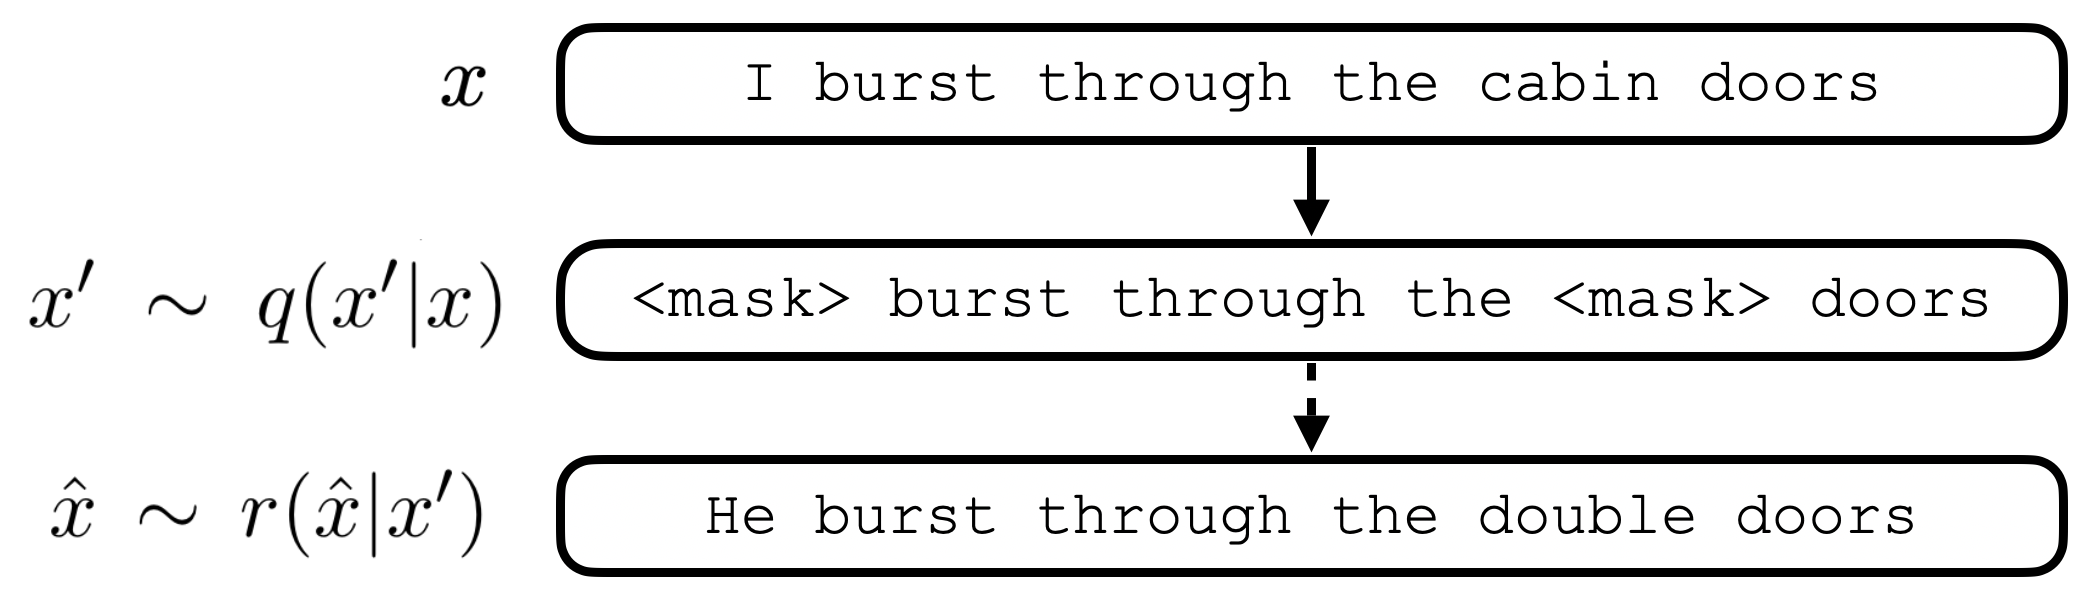
\includegraphics[scale=0.21]{img/bert_dae.png}
\caption{To sample from an MLM DAE, we apply the MLM corruption $q$ to the original sentence then reconstruct the corrupted sentence using our DAE $r$.}
\label{fig:dae_sampling}
\end{figure}

\subsection{Sampling from Denoising Autoencoders}
A denoising autoencoder (DAE) is an autoencoder trained to reconstruct a clean input $x$ from a stochastically corrupted one $x'\sim q(x'|x)$ by learning a conditional distribution $P_\theta (x| x')$ \citep{vincent2008extracting}.
We can sample from a DAE by successively corrupting and reconstructing an input using the following pseudo-Gibbs Markov chain: $x_t' \sim q(x'|x_{t-1})$, $x_t \sim P_\theta(x|x'_t).$
\comment{
\begin{align*}
    x_t' &\sim q(x'|x_{t-1})\\
    x_t &\sim P_\theta(x|x'_t) 
\end{align*}
}
As the number of training examples increases, the asymptotic distribution $\pi_n(x)$ of the generated samples approximate the true data-generating distribution $P(x)$ \citep{bengio2013generalized}.
This corruption-reconstruction process allows for sampling directly along the manifold that $P(x)$ concentrates on.

\subsection{Masked Language Models}
Recent advances in unsupervised representation learning for natural language have relied on pre-training models on a \textit{masked language modeling} (MLM) objective \citep{devlin2018, liu2019roberta}.
In the MLM objective, a percentage of the input tokens are randomly corrupted and the model is asked to reconstruct the original token given its left and right context in the corrupted sentence.
We use MLMs as DAEs \citep{lewis2019bart} to sample from the underlying natural language distribution by corrupting and reconstructing inputs (Figure \ref{fig:dae_sampling}).


\section{FlashAttention-3: Algorithm}
\label{sec:algo}

In this section, we describe the \fat algorithm. For simplicity, we focus on the
forward pass, with the backward pass algorithm described in~\cref{sec:algo_ws_bwd}. We first indicate how to integrate warp-specialization with a circular SMEM buffer into the base algorithm of \faa. We then explain how to exploit asynchrony of WGMMA to define an overlapped GEMM-softmax 2-stage pipeline. Finally, we describe the modifications needed for FP8, both in terms of layout conformance and accuracy via block quantization and incoherent processing.

\subsection{Producer-Consumer asynchrony through warp-specialization and
  pingpong scheduling}
\label{sec:algo_ws}

\paragraph{Warp-specialization}
As with \faa, the forward pass of \fat is embarrassingly parallel in the batch size, number of heads, and query sequence length.
Thus, it will suffice to give a CTA-level view of the algorithm, which operates on a tile $\vQ_i$ of the query matrix to compute the corresponding tile $\vO_i$ of the output.
To simplify the description, we first give the warp-specialization scheme with a circular SMEM buffer that does \emph{not} have in addition the GEMM-softmax overlapping.
Let $d$ be the head dimension, $N$ the sequence length, and fix a query block size $B_r$ to divide $\vQ$ into $T_r = \lceil \frac{N}{B_r} \rceil$ blocks $\vQ_1, .., \vQ_{T_r}$.

\begin{algorithm}[H]
    \caption{\small\label{alg:flash3_wgmma_ws_only}\fat forward pass \textbf{without} intra-consumer overlapping -- CTA view}
    \begin{algorithmic}[1]
\REQUIRE Matrices $\vQ_i \in \RR^{B_r \times d}$ and $\vK, \vV \in \mathbb{R}^{N \times d}$ in HBM, key block size $B_c$ with $T_c = \lceil \frac{N}{B_c} \rceil$.
\STATE Initialize pipeline object to manage barrier synchronization with $s$-stage circular SMEM buffer.
\IF {in producer warpgroup}
\STATE Deallocate predetermined number of registers.
\STATE Issue load $\vQ_i$ from HBM to shared memory.
\STATE Upon completion, commit to notify consumer of the load of $\vQ_i$.
\FOR{$0 \le j < T_c$}
    \STATE Wait for the $(j\,\%\,s)$th stage of the buffer to be consumed.
    \STATE Issue loads of $\vK_j, \vV_j$ from HBM to shared memory at the $(j\,\%\,s)$th stage of the buffer.
    \STATE Upon completion, commit to notify consumers of the loads of $\vK_j, \vV_j$.
\ENDFOR
\ELSE
\STATE Reallocate predetermined number of registers as function of number of consumer warps.
\STATE On-chip, initialize $\vO_i = (0) \in \mathbb{R}^{B_r \times d}$ and $\ell_i, m_i = (0), (-\infty) \in \mathbb{R}^{B_r}$.
\STATE Wait for $\vQ_i$ to be loaded in shared memory.
\FOR{$0 \le j < T_c$}
\STATE Wait for $\vK_j$ to be loaded in shared memory.
\STATE Compute $\vS_i^{(j)} = \vQ_i \vK_j^T$ (SS-GEMM). Commit and wait. \label{alg:ws_only_gemm1}
\STATE Store $m_i^{\mathrm{old}} = m_i$ and compute $m_i = \max(m_i^{\mathrm{old}}, \rowmax(\vS_i^{(j)}))$. \label{code-ws:softmax_start}
\STATE Compute $\widetilde{\vP}_i^{(j)} = \exp(\vS_i^{(j)} - m_i)$ and $\ell_i = \exp(m_i^{\mathrm{old}} - m_i) \ell_i + \rowsum(\widetilde{\vP}_i^{(j)})$. \label{code-ws:softmax_end}
\STATE Wait for $\vV_j$ to be loaded in shared memory.
\STATE Compute $\vO_i = \diag(\exp(m_i^{\mathrm{old}} - m_i))^{-1} \vO_i + \widetilde{\vP}_i^{(j)} \vV_j$ (RS-GEMM). Commit and wait. \label{alg:ws_only_gemm2}
\STATE Release the $(j\,\%\,s)$th stage of the buffer for the producer.
\ENDFOR
\STATE Compute $\vO_i = \diag(\ell_i)^{-1} \vO_i$ and $L_i = m_i + \log(\ell_i)$.
\STATE Write $\vO_i$ and $L_i$ to HBM as the $i$th block of $\vO$ and $L$.
\ENDIF
\end{algorithmic}
\end{algorithm}

For our implementation of \cref{alg:flash3_wgmma_ws_only} on Hopper, we use \verb|setmaxnreg| for (de)allocations, TMA for loads of $\vQ_i$ and $\{ \vK_j, \vV_j \}_{0 \leq j < T_c}$, and WGMMA to execute the GEMMs in the consumer mainloop, with the SS or RS prefix indicating whether the first operand is sourced from shared memory or register file.
For interpreting the execution flow of \cref{alg:flash3_wgmma_ws_only}, note that issuing TMA loads does not stall on the completion of other loads due to asynchrony.
Moreover, in the producer mainloop, no waits will be issued for the first $s$ iterations as the buffer gets filled.

\paragraph{Pingpong scheduling}
The asynchronous nature of WGMMA and TMA, along with warp-specialization, opens
up the opportunity to overlap the softmax computation of one warpgroup with the GEMM of
another warpgroup.
To motivate this, notice that non-matmul operations have much lower throughput
than matmul operations on modern hardware accelerators.
As an example, the H100 SXM5 GPU has 989 TFLOPS of FP16 matmul but only 3.9
TFLOPS of special functions such as exponential\footnote{The CUDA programming
  guide specifies that 16 operations of special functions can be performed per
  streaming multiprocessor (SM) per clock cycle. We multiply 16 by 132 SMs and
  1830 MHz clock speed to get 3.9 TFLOPS of special functions.} (necessary for softmax).
For the attention forward pass in FP16 with head dimension 128, there are 512x more matmul FLOPS
compared to exponential operations, but the exponential has 256x lower
throughput, so exponential can take 50\% of the cycle compared to matmul.
The situation is even worse with FP8, where the matmul throughput doubles but
the exponential throughput stays the same.

Since the exponential is performed by a separate hardware unit (the multi-function
unit), ideally we'd want the exponential calculation to be scheduled when the
Tensor Cores are performing the matmul.
To do so, we use synchronization barriers (\texttt{bar.sync} instructions) to
force the GEMMs (GEMM1 -- $\vP \vV$ of one iteration, and GEMM0 -- $\vQ \vK^\top$
of the next iteration) of warpgroup 1 to be scheduled before the GEMMs of
warpgroup 2.
As a result, the softmax of warpgroup 1 will be scheduled while warpgroup 2 is
performing its GEMMs. Then the roles swap, with warpgroup 2 doing softmax while
warpgroup 1 doing GEMMs (hence, ``pingpong'' scheduling).
This is illustrated in~\cref{fig:pingpong_scheduling}.
Though in practice the pingpong scheduling is not as clean as depicted in the
figure, we generally find this to improve performance (e.g., from 570 TFLOPS to
620-640 TFLOPS for FP16 forward with head dimension 128 and sequence length 8192).
\begin{figure}[ht]
    \centering
    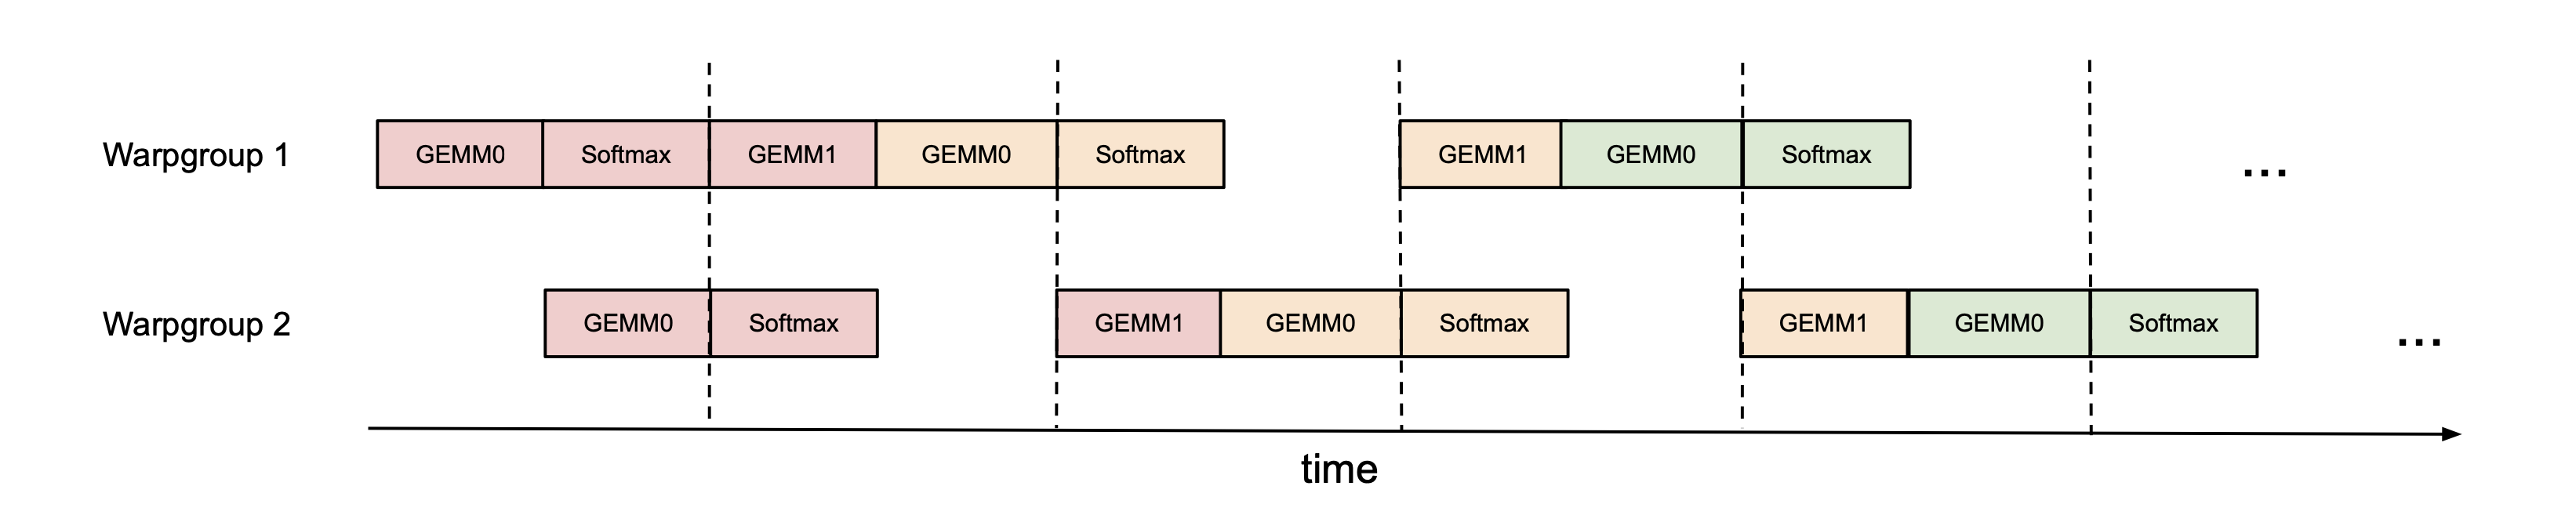
\includegraphics[width=1.0\linewidth]{figs/pingpong_pipelining.png}
    \caption{Pingpong scheduling for 2 warpgroups to overlap softmax and GEMMs: the softmax of one warpgroup
      should be scheduled when the GEMMs of another warpgroup are running. The
      same color denotes the same iteration.}
    \label{fig:pingpong_scheduling}
\end{figure}

\paragraph{Attention variants}
For multi-query attention~\citep{shazeer2019fast} and grouped query
attention~\citep{ainslie2023gqa}, we follow the approach in \faa and adjust the
tensor indexing to avoid duplicating $\vK$ and $\vV$ in HBM.

\subsection{Intra-warpgroup overlapping GEMMs and softmax}


Even within one warpgroup, we can overlap some instructions in the softmax with
some instructions in the GEMMs. We describe one technique to do so.

In the attention algorithm, operations within the inner loop (main loop) have sequential dependencies that impede parallelization within a single iteration.
For example, (local) softmax (lines \ref{code-ws:softmax_start} to \ref{code-ws:softmax_end}) relies on the output $\vS_i^{(j)}$ of the first GEMM, while the second GEMM takes its result $\widetilde{\vP}_i^{(j)}$ as an operand.
Indeed, the wait statements in lines \ref{alg:ws_only_gemm1} and \ref{alg:ws_only_gemm2} of \cref{alg:flash3_wgmma_ws_only} serialize the execution of softmax and GEMMs.
However, we can break these dependencies by pipelining across iterations through additional buffers in registers.
Pursuing this idea, we propose the following two-stage\footnote{Note that the number of stages of the overlapping scheme is bounded by, but need not equal, the number $s$ of stages in the circular SMEM buffer.} GEMM-softmax pipelining algorithm:

\begin{figure}[ht]
    \centering
    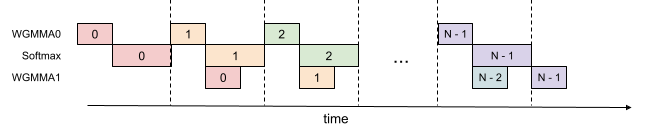
\includegraphics[width=.95\linewidth]{figs/2_stage_pipelining.png}
    \caption{2-stage WGMMA-softmax pipelining}
    \label{fig:2_stage_pipelining}
\end{figure}

\begin{algorithm}[H]
    \caption{\small\label{alg:flash3_wgmma}\fat consumer warpgroup forward pass}
    \begin{algorithmic}[1]
      \REQUIRE  Matrices $\vQ_i \in \RR^{B_r \times d}$ and $\vK, \vV \in \mathbb{R}^{N \times d}$ in HBM, key block size $B_c$ with $T_c = \lceil \frac{N}{B_c} \rceil$.
      \STATE Reallocate predetermined number of registers as function of number of consumer warps.
      \STATE On-chip, initialize $\vO_i = (0) \in \mathbb{R}^{B_r \times d}$ and $\ell_i, m_i = (0), (-\infty) \in \mathbb{R}^{B_r}$.
      \STATE Wait for $\vQ_i$ and $\vK_0$ to be loaded in shared memory.
      \STATE Compute $\vS_{\mathrm{cur}} = \vQ_i \vK_0^T$ using WGMMA. Commit and wait.
      \STATE Release the $0$th stage of the buffer for $\vK$.
      \STATE Compute $m_{i}$, $\tilde{\vP}_{\mathrm{cur}}$ and $\ell_{i}$ based on $\vS_{\mathrm{cur}}$, and rescale $\vO_i$.
      \FOR{$1 \le j < T_c - 1$}
        \STATE Wait for $\vK_j$ to be loaded in shared memory.
        \label{code:mainloop_start}
        \STATE Compute $\vS_{\mathrm{next}} = \vQ_i \vK_{j}^T$ using WGMMA. Commit but do not wait. \label{code:first_wgmma}
        \STATE Wait for $\vV_{j-1}$ to be loaded in shared memory.
        \STATE Compute $\vO_{i} = \vO_{i} + \tilde{\vP}_{\mathrm{cur}} \vV_{j-1}$ using WGMMA. Commit but do not wait. \label{code:second_wgmma}
        \STATE Wait for the WGMMA $\vQ_i \vK_{j}^T$.
        \STATE Compute $m_{i}$, $\tilde{\vP}_{\mathrm{next}}$ and $\ell_{i}$ based on $\vS_{\mathrm{next}}$. \label{code:softmax}
        \STATE Wait for the WGMMA $\tilde{\vP}_{\mathrm{cur}} \vV_{j-1}$ and then rescale $\vO_i$
        \STATE Release the $(j\,\%\,s)$th, resp. $(j-1\,\%\,s)$th stage of the buffer for $\vK$, resp. $\vV$.
        \STATE Copy $\vS_{\mathrm{next}}$ to $\vS_{\mathrm{cur}}$.
        \label{code:mainloop_end}
      \ENDFOR
      \STATE Wait for $\vV_{T_c - 1}$ to be loaded in shared memory.
      \STATE Compute
      $\vO_{i} = \vO_{i} + \tilde{\vP}_{\mathrm{last}} \vV_{T_c - 1}$ using WGMMA. Commit and wait.

      \STATE Epilogue:
      Rescale $\vO_{i}$ based on $m_{i}$.
      Compute $L_{i}$ based on $m_{i}$ and $\ell_{i}$.
      Write $\vO_{i}$ and $L_{i}$ to HBM as the $i$-th block of $\vO$ and $L$.
    \end{algorithmic}
  \end{algorithm}

  \cref{alg:flash3_wgmma} functions as a replacement for the consumer path of \cref{alg:flash3_wgmma_ws_only} to comprise the complete \fat algorithm for FP16 precision. At a high-level, we use WGMMA as a metonym for asynchronous GEMM. Within the mainloop (lines \ref{code:mainloop_start} to \ref{code:mainloop_end}), the second WGMMA operation of iteration $j$ (line \ref{code:second_wgmma}) is overlapped with softmax operations from iteration $j+1$ (line \ref{code:softmax}).

  While the pipelined structure illustrated above offers theoretical performance gains, there are several practical aspects to consider:
  \paragraph{Compiler reordering}
  The pseudocode represents an idealized execution order but the compiler (NVCC) often rearranges instructions for optimization.
  This can disrupt the carefully crafted WGMMA and non-WGMMA operation pipelining sequence, potentially leading to unexpected behavior or diminished performance gains. An analysis of the SASS code shows that the compiler generates overlapped code as expected (Section~\ref{sec:2-stage-sass}).
  \paragraph{Register pressure}
  To maintain optimal performance, register spilling should be minimized.
  However, the 2-stage pipeline requires additional registers to store intermediate results and maintain context between stages.
  Specifically, an extra $\vS_{\mathrm{next}}$ must be kept in registers, leading to extra register usage of size $B_r \times B_c \times \text{sizeof}(\text{float})$ per threadblock.
  This increased register demand may conflict with using larger block sizes (another common optimization), which is also register-hungry.
  In practice, trade-offs should be made based on profiling results.
  \paragraph{3-stage pipelining} Extending the 2-stage algorithm described above, we propose a 3-stage variant
  that would further overlap the second WGMMA with softmax.
  While this approach offers the potential for even higher Tensor Core utilization,
  it requires even more registers due to an additional stage in the pipeline,
  making the trade-off between tile size and pipeline depth more difficult to balance.
  A detailed description of the 3-stage algorithm and its evaluation results can be found in ~\cref{sec:3-stage}.

\subsection{Low-precision with FP8}
\label{sec:algofp8}

\begin{figure} %
\centering
\begin{tikzpicture}
\definecolor{mygold}{RGB}{255, 215, 0} %
\definecolor{warmcolor}{RGB}{255, 165, 0} %
\def\r{.9}
\def\h{-.5}
\foreach \y in {0,2} {
  \ifnum\y=0
    \def\mycolor{cyan!20}
  \else
    \def\mycolor{mygold!20}
  \fi
  \foreach \x in {0,2} {
    \draw[fill=\mycolor] (4*\y*\r+\x*\r,0) rectangle ++(2*\r,.5);
    \draw[fill=\mycolor] (4*\r+4*\y*\r+\x*\r,0) rectangle ++(2*\r,.5);
  }
}
\foreach \y in {0,2} {
  \ifnum\y=0
    \def\mycolor{cyan!50}
  \else
    \def\mycolor{warmcolor!50}
  \fi
  \foreach \x in {0,2} {
    \draw[fill=\mycolor] (4*\y*\r+\x*\r,\h) rectangle ++(2*\r,.5);
    \draw[fill=\mycolor] (4*\r+4*\y*\r+\x*\r,\h) rectangle ++(2*\r,.5);
  }
}

\foreach \y in {0,2} {
  \foreach \x in {0} {
    \ifnum\y=0
      \node at (4*\y*\r+\x*\r + \r, 0.25) {T0\,\{d0,\,d1\}};
    \else
      \node at (4*\y*\r+\x*\r + \r, 0.25) {T0\,\{d4,\,d5\}};
    \fi
  }
  \foreach \x in {2} {
    \ifnum\y=0
      \node at (4*\y*\r+\x*\r + \r, 0.25) {T1\,\{d0,\,d1\}};
    \else
      \node at (4*\y*\r+\x*\r + \r, 0.25) {T1\,\{d4,\,d5\}};
    \fi
  }
}
\foreach \y in {1,3} {
  \foreach \x in {0} {
  \ifnum\y=1
    \node at (4*\y*\r+\x*\r + \r, 0.25) {T2\,\{d0,\,d1\}};
  \else
    \node at (4*\y*\r+\x*\r + \r, 0.25) {T2\,\{d4,\,d5\}};
  \fi
  }
  \foreach \x in {2} {
  \ifnum\y=1
    \node at (4*\y*\r+\x*\r + \r, 0.25) {T3\,\{d0,\,d1\}};
  \else
    \node at (4*\y*\r+\x*\r + \r, 0.25) {T3\,\{d4,\,d5\}};
  \fi
  }
}

\foreach \y in {0,2} {
    \foreach \x in {0} {
      \ifnum\y=0
        \node at (4*\y*\r+\x*\r + \r, 0.25+\h) {T0\,\{d2,\,d3\}};
      \else
        \node at (4*\y*\r+\x*\r + \r, 0.25+\h) {T0\,\{d6,\,d7\}};
      \fi
    }
    \foreach \x in {2} {
      \ifnum\y=0
        \node at (4*\y*\r+\x*\r + \r, 0.25+\h) {T1\,\{d2,\,d3\}};
      \else
        \node at (4*\y*\r+\x*\r + \r, 0.25+\h) {T1\,\{d6,\,d7\}};
      \fi
    }
  }

\foreach \y in {1,3} {
  \foreach \x in {0} {
  \ifnum\y=1
    \node at (4*\y*\r+\x*\r + \r, 0.25+\h) {T2\,\{d2,\,d3\}};
  \else
    \node at (4*\y*\r+\x*\r + \r, 0.25+\h) {T2\,\{d6,\,d7\}};
  \fi
  }
  \foreach \x in {2} {
  \ifnum\y=1
    \node at (4*\y*\r+\x*\r + \r, 0.25+\h) {T3\,\{d2,\,d3\}};
  \else
    \node at (4*\y*\r+\x*\r + \r, 0.25+\h) {T3\,\{d6,\,d7\}};
  \fi
  }
}
\end{tikzpicture}
\caption{FP32 accumulator register WGMMA layout -- rows 0 and 8, threads 0-3, entries 0-7.}
\label{fig:rmem_accum}
\end{figure}

\begin{figure}
\centering
\begin{tikzpicture}
\definecolor{mygold}{RGB}{255, 215, 0} %
\definecolor{warmcolor}{RGB}{255, 165, 0} %
\def\r{.9}
\def\h{-.5}

\foreach \y in {0,...,3} {
  \foreach \x in {0,2} {
    \ifnum\x=0
      \def\mycolor{cyan!20}
    \else
      \def\mycolor{cyan!50}
    \fi
    \draw[fill=\mycolor] (4*\y*\r+\x*\r,0) rectangle ++(2*\r,.5);
  }
}
\foreach \y in {0,...,3} {
  \foreach \x in {0,2} {
    \ifnum\x=0
      \def\mycolor{mygold!20}
    \else
      \def\mycolor{warmcolor!50}
    \fi
    \draw[fill=\mycolor] (4*\y*\r+\x*\r,\h) rectangle ++(2*\r,.5);
  }
}
\foreach \y in {0,...,3} {
    \foreach \x in {0,2} {
      \ifnum\x=0
        \node at (4*\y*\r+\x*\r + \r, 0.25) {T\y\,\{a0,\,a1\}};
      \else
        \node at (4*\y*\r+\x*\r + \r, 0.25) {T\y\,\{a2,\,a3\}};
      \fi
    }
}
\foreach \y in {0,...,3} {
    \foreach \x in {0,2} {
      \ifnum\x=0
        \node at (4*\y*\r+\x*\r + \r, 0.25+\h) {T\y\,\{a4,\,a5\}};
      \else
        \node at (4*\y*\r+\x*\r + \r, 0.25+\h) {T\y\,\{a6,\,a7\}};
      \fi
    }
}
\end{tikzpicture}
\caption{FP8 operand A register WGMMA layout -- rows 0 and 8, threads 0-3, entries 0-7.}
\label{fig:rmem_operand}
\end{figure}

\textbf{Efficiency: layout transformations.}
Computing the forward pass of \fat in FP8 precision poses additional challenges not encountered for FP16 in terms of layout conformance.

First, we note that the input tensors $\vQ$, $\vK$, and $\vV$
are typically given as contiguous in the head dimension,
while to satisfy the k-major constraint on FP8 WGMMA for the second GEMM we need $\vV$,
or rather the tiles of $\vV$ loaded into SMEM, to be contiguous in the sequence length dimension.
Since the TMA load itself cannot change the contiguous dimension, we then need to either
(1) transpose $\vV$ in GMEM as a pre-processing step, or
(2) do an in-kernel transpose of tiles of $\vV$ after loading them into SMEM.
To implement option (1), we can either
(1a) fuse the transpose to the epilogue of a preceding step such as the rotary embedding, or
(1b) call a standalone pre-processing transpose
kernel\footnote{An optimized transpose kernel will achieve speed near the bandwidth of the device~\citep{colfax_cutlass_transpose_2024}.}
to exchange the strides of the sequence length and head dimensions.
However, (1a) is difficult to integrate into a standard library,
and (1b) is too wasteful in a memory-bound situation such as inference.

Instead, for FP8 \fat we opt for option (2).
For the in-kernel transpose, we take advantage of the LDSM (\verb|ldmatrix|)
and STSM (\verb|stmatrix|) instructions,
which involve a warp of threads collectively loading SMEM to RMEM
and storing RMEM to SMEM at a granularity of 128 bytes.\footnote{In the PTX documentation, LDSM/STSM are described as copying $8 \times 8$ matrices with 16-bit entries \cite[\S 9.7.13.4.15-16]{ptx},
but we can pack 8-bit entries two at a time to use LDSM/STSM in the context of FP8 precision.
However, the transpose versions of LDSM/STSM cannot split packed 8-bit entries,
which necessitates certain register movements in between LDSM and STSM to actually perform a tile-wise transpose; we omit the details.}
The LDSM/STSM instructions are both register efficient,
allowing us to execute them in the producer warpgroup,
and capable of transposing layouts when doing memory copy.
Moreover, after the first iteration we can arrange
for the transpose of the next $\vV$ tile
to be executed in the shadow of the two WGMMAs
that involve the preceding $\vV$ and current $\vK$ tile.

Second, we observe that unlike with FP16,
the memory layout of the FP32 accumulator of an FP8 WGMMA is different
from that assumed for its operand A when held in registers.
We depict fragments of these two layouts in \cref{fig:rmem_accum} and \cref{fig:rmem_operand},
where the entries are held in registers per thread in the listed order.
By using byte permute instructions,
we can then transform the first WGMMA's accumulator into a format suitable for the second WGMMA,
and compatibly with the layout of the $\vV$ tile produced by the in-kernel transpose. Specifically, with reference to \cref{fig:rmem_accum}, we change the order in sequence to
$$\{ \verb|d0 d1 d4 d5 d2 d3 d6 d7| \},$$
and this register permutation is then replicated over every 8 bytes. In terms of the logical shape of the $\vP$ tile, this manuever permutes its columns (e.g., columns $0189$ now become the first four columns). For WGMMA to then compute the correct output tile, we can correspondingly arrange for the in-kernel transpose to write out a matching row permutation of the $\vV$ tile.\footnote{This additional freedom afforded by doing the in-kernel transpose eliminates having to use shuffle instructions to change register ownership across threads, which we previously described in~\citep{colfax_fp8_flashattention_2024}.}






\textbf{Accuracy: block quantization and incoherent processing.}
With FP8 (e4m3) format, one only uses 3 bits to store the mantissa and 4 bits
for the exponent.
This results in higher numerical error than FP16/BF16.
Moreover, large models typically have outlier values~\citep{dettmers2208llm,
  sun2024massive} that are much larger in magnitude than most other values,
making quantization difficult.
One typically use per-tensor scaling~\citep{micikevicius2022fp8} by keeping one scalar per tensor (e.g., one
for $\vQ$, for $\vK$, and for $\vV$).
To reduce the numerical error of attention in FP8, we employ two techniques:
\iftoggle{arxiv}{
\begin{enumerate}
}{
\begin{enumerate}[itemsep=0pt,topsep=0pt,leftmargin=*]
}
\item \textbf{Block quantization}: we keep one scalar per block, so that
 for each of $\vQ$, $\vK$, $\vV$ we split the tensor into blocks of
  size $B_r \times d$ or $B_c \times d$ and quantize them separately.
  This quantization can be fused with an operation right before attention (e.g.,
  rotary embedding) with no additional slow down (since rotary embedding is
  memory-bandwidth bound).
  As the \fat algorithm naturally operates on blocks, we can scale each block of
  $\vS$ to account for this block quantization at no computation cost.
\item \textbf{Incoherent processing}: to even out outliers, we multiply
  $\vQ$ and $\vK$ with a random orthogonal matrix $\vM$ before quantizing to
  FP8. Since $\vM$ is orthogonal, $\vM \vM^\top = I$ and so $(\vQ \vM) (\vK
  \vM)^\top = \vQ \vK^\top$, i.e., multiplying both $\vQ$ and $\vK$ with
  $\vM$ does not change the attention output.
  This serves to ``spread out'' the outliers since each entry of $\vQ \vM$
  or $\vK \vM$ is a random sum of entries of $\vQ$ or $\vK$, thus reducing
  quantization error.
  In practice, we follow \citet{chee2024quip} and~\citet{tseng2024quip} and choose $\vM$ to be the product of random diagonal matrices of $\pm
  1$ and a Hadamard matrix, which can be multiplied in $O(d \log d)$ instead of
  $O(d^2)$, and can also be fused with the rotary embedding at no extra computation cost.
\end{enumerate}
We validate that these two techniques reduces numerical error by up to 2.6$\times$ in \cref{sec:numerical_error}.


\vspace{-0.2cm}
\section{Experiments Details}
\label{sec:exp}

\vspace{-0.2cm}
\subsection{Roadmap Insights on FFHQ-256\texorpdfstring{~\cite{sg1}}{}}
\label{sub:arc-experiments}
\vspace{-0.1cm}
As per Table~\ref{tab:roadmap}, Config A (vanilla StyleGAN2) achieves an FID of 7.52 using the official implementation on FFHQ-256. Config B with all tricks removed achieves an FID of 12.46---performance drops as expected. 
Config C, with a well-behaved loss, achieves an FID of 11.65. But, now training is sufficiently stable to improve the architecture.

Config D, which improves $G$ and $D$ based on the classic ResNet and ConvNeXt findings, achieves an FID of 9.95. The output skips of the StyleGAN2 generator are no longer useful given our new architecture; including them produces a worse FID of 10.17. Karras~\etal find that the benefit of output skips is mostly related to gradient magnitude dynamics~\cite{sg3}, and this has been addressed by our ResNet architecture. For StyleGAN2, Karras~\etal conclude that a ResNet architecture is harmful to $G$~\cite{sg2}, but this is not true in our case as their ResNet implementation is considerably different from ours: 1) Karras~\etal use one 3-3 residual block for each resolution stage, while we have a separate transition layer and two 1-3-1 residual blocks; 2) i.3) and i.4) are violated as they do not have a linear residual block~\cite{mobnet} and the transition layer is placed on the skip branch of the residual block rather than the stem; 3) the essential principle of ResNet~\cite{resnet}---identity mapping~\cite{resnet2}---is violated as Karras~\etal divide the output of the residual block by $\sqrt{2}$ to avoid variance explosion due to the absence of a proper initialization scheme.

For Config E, we conduct two experiments that ablate i.\ref{item:i1} (increased width with depthwise conv.) and i.\ref{item:i2} (an inverted bottleneck). We add GroupedConv and reduce the bottleneck compression ratio to two given the same model size. Each bottleneck is now 1.5$\times$ the width of Config A, and the FID drops to 7.51, surpassing the performance of StyleGAN2. By inverting the stem and the bottleneck dimensions to enhance the capacity of GroupedConv, our final model achieves an FID of 7.05, exceeding StyleGAN2.


\begin{wraptable}[12]{r}{6.5cm}
\vspace{-1.25cm}
\centering
\caption{StackedMNIST 1000-mode coverage.}
% Our model outperforms other GANs in terms of $D_\text{KL}$, indicating that we are better able to recover the distribution.}
\vspace{-0.4cm}
\resizebox{0.8\linewidth}{!}{
\begin{tblr}{
  cell{2}{2} = {c},
  cell{2}{3} = {c},
  cell{3}{2} = {c},
  cell{3}{3} = {c},
  cell{4}{2} = {c},
  cell{4}{3} = {c},
  cell{5}{2} = {c},
  cell{5}{3} = {c},
  cell{6}{2} = {c},
  cell{6}{3} = {c},
  cell{7}{2} = {c},
  cell{7}{3} = {c},
  cell{8}{2} = {c},
  cell{8}{3} = {c},
  cell{9}{2} = {c},
  cell{9}{3} = {c},
  cell{10}{2} = {c},
  cell{10}{3} = {c},
  cell{11}{2} = {c},
  cell{11}{3} = {c},
  cell{12}{2} = {c},
  cell{12}{3} = {c},
  hline{2,12} = {1-3}{},
}
Model     & \# modes$\uparrow$ & $D_\text{KL}$$\downarrow$            &  \\
DCGAN~\cite{dcgan}     & 99            & 3.40\phantom{0}&  \\
VEEGAN~\cite{srivastava2017veegan}    & 150           & 2.95\phantom{0}&  \\
WGAN-GP~\cite{wgan-gp}& 959           & 0.73\phantom{0}&  \\
PacGAN~\cite{pacgan}    & 992           & 0.28\phantom{0}&  \\
StyleGAN2~\cite{sg2} & 940           & 0.42\phantom{0}&  \\
PresGAN~\cite{presgan}   & \textbf{1000} & 0.12\phantom{0}&  \\
Adv. DSM~\cite{advsm}  & \textbf{1000} & 1.49\phantom{0}&  \\
VAEBM~\cite{vaebm}     & \textbf{1000} & 0.087          &  \\
DDGAN~\cite{ddgan}     & \textbf{1000} & 0.071          &  \\
MEG~\cite{meg}       & \textbf{1000} & 0.031          &  \\
Ours---Config E     & \textbf{1000} & \textbf{0.029} &  
\end{tblr}
}
\label{tab:stackedmnist}
\end{wraptable}%

\subsection{Mode Recovery --- StackedMNIST\texorpdfstring{~\cite{metz2016unrolled}}{}} 
\vspace{-0.1cm}
We repeat the earlier experiment in 1000-mode convergence on StackedMNIST (unconditional generation), but this time with our updated architecture and with comparisons to SOTA GANs and likelihood-based methods (Tab.~\ref{tab:stackedmnist}, Fig.~\ref{fig:stacked-mnist}). 
One advantage brought up of likelihood-based models such as diffusion over GANs is that they achieve mode coverage~\cite{adm}. We find that most GANs struggle to find all modes. But, PresGAN~\cite{presgan}, DDGAN~\cite{ddgan}, and our approach are successful. Further, our method outperforms all other tested GAN models in term of KL divergence.

\subsection{FID --- FFHQ-256\texorpdfstring{~\cite{sg1}}{} (Optimized)}
\vspace{-0.1cm}
We train Config E model until convergence and with optimized hyperparameters and training schedule on FFHQ at 256$\times$256 (unconditional generation) (Tab.~\ref{tab:ffhq256}, Figs.~\ref{fig:ffhq-256-teaser} and~\ref{fig:ffhq-256}). 
Please see our supplemental material for training details.
%The hyperparameters and schedule are listed in the supplemental material. 
Our model outperforms existing StyleGAN methods, plus four more recent diffusion-based methods. On this common dataset experimental setting, many methods (not listed here) use the bCR~\cite{zhao2021improved} trick---this has only been shown to improve performance on FFHQ-256 (not even at different resolutions of FFHQ)~\cite{zhao2021improved, zhang2022styleswin}. We do not use this trick. 
% no such tricks in our method.
% JT Try to minimize embellishment...
% This is particularly impressive given the fact that the dataset FFHQ was designed for StyleGAN~\cite{sg1} and the StyleGAN series of models were optimized with this specific dataset in mind.
% to achieve this performance.

\subsection{FID --- FFHQ-64\texorpdfstring{~\cite{edm}}{}}
\vspace{-0.1cm}
To compare with EDM~\cite{edm} directly, we evaluate our model on FFHQ at 64$\times$64 resolution. For this, we remove the two highest resolution stages of our 256$\times$256 model, resulting in a generator that is less than half the number of parameters as EDM. Despite this, our model outperforms EDM on this dataset and needs one function evaluation only (Tab.~\ref{tab:ffhq64}).

\begin{figure}
\begin{floatrow}
    %\hspace{-0.75cm}%
    \capbtabbox{%
        \centering
        \resizebox{\linewidth}{!}{
        \begin{tblr}{
          column{2,3} = {r},
          cell{1}{2} = {c},
          cell{1}{3} = {c},
          hline{2,5,9,10} = {-}{},
        }
        Model       & NFE$\downarrow$ & FID$\downarrow$  \\
        StyleGAN2~\cite{sg2}   & 1               & 3.78 \\
        StyleGAN3-T~\cite{sg3} & 1               & 4.81 \\
        StyleGAN3-R~\cite{sg3} & 1               & 3.92 \\
        LDM~\cite{rombach2022high} & 200               & 4.98\\
        ADM (DDIM)~\cite{adm,compdiff} & 500               & 8.41\\
        ADM (DPM-Solver)~\cite{adm,compdiff} & 500               & 8.40\\
        Diffusion Autoencoder~\cite{diffae,compdiff} & 500               & 5.81\\
        Ours---Config E  & 1               & 2.75 \\
        \emph{With ImageNet feature leakage~\cite{kynkaanniemi2022role}:} & & \\
        PolyINR*~\cite{singh2023polynomial} & 1               & 2.72 \\
        StyleGAN-XL*~\cite{sgxl} & 1               & 2.19 \\
        StyleSAN-XL*~\cite{takida2024san} & 1               & 1.68 \\
        \end{tblr}
        }
    }{%
        \caption{
        \label{tab:ffhq256}FFHQ-256. * denotes models that leak ImageNet features.}
    }
    %
    \capbtabbox{%
        \centering
        \resizebox{0.85\linewidth}{!}{
        \begin{tblr}{
          column{2} = {r},
          column{3} = {r},
          hline{2,5,8} = {-}{},
        }
        Model         & NFE$\downarrow$ & FID$\downarrow$ \\
        StyleGAN2~\cite{sg2,anycostgan}     & 1               & 3.32            \\
        MSG-GAN~\cite{karnewar2020msg,anycostgan}       & 1               & 2.7             \\
        Anycost GAN~\cite{anycostgan}   & 1               & 2.52            \\
        VE~\cite{sde,edm}            & 79              & 25.95           \\
        VP~\cite{sde,edm}            & 79              & 3.39            \\
        EDM~\cite{edm}           & 79              & 2.39            \\
        Ours—Config E & 1               & 1.95 \\
        \end{tblr}
        }
    }{%
        \caption{\label{tab:ffhq64}FFHQ-64.}
    }
\end{floatrow}
\vspace{-0.25cm}
\end{figure}


% \begin{figure}
% \begin{floatrow}
%     \capbtabbox{%
%         \centering
%         \resizebox{0.8\linewidth}{!}{
%         \begin{tblr}{
%           column{2,3} = {r},
%           cell{1}{2} = {c},
%           cell{1}{3} = {c},
%           hline{2,9,13} = {-}{},
%         }
%         Model               & NFE$\downarrow$ & FID$\downarrow$ \\
%         BigGAN~\cite{biggan}              & 1               & 14.73 \\
%         TransGAN~\cite{trans}            & 1               & 9.26 \\
%         ViTGAN~\cite{vitgan}              & 1               & 6.66 \\
%         DDGAN~\cite{ddgan}               & 4               & 3.75 \\
%         Diffusion StyleGAN2~\cite{diffusiongan} & 1               & 3.19 \\
%         StyleGAN2 + ADA~\cite{sg2ada}     & 1               & 2.42 \\
%         StyleGAN3-R + ADA~\cite{sg3,studio}   & 1               & 10.83 \\
%         DDPM~\cite{ddpm}               & 1000            & 3.21 \\
%         DDIM~\cite{ddim}                & 50             & 4.67 \\
%         VE~\cite{sde,edm}                  & 35              & 3.11 \\
%         VP~\cite{sde,edm}                  & 35              & 2.48 \\
%         Ours---Config E     & 1               & 1.96 \\
%         \hline
%         \emph{With ImageNet feature leakage~\cite{kynkaanniemi2022role}:} & & \\
%         StyleGAN-XL*~\cite{sgxl}       & 1               & 1.85 \\
%         \end{tblr}
%         }
%     }{%
%         \caption{\label{tab:cifar10}CIFAR-10.}
%     }
%         % \begin{tblr}{
%         %   column{2,3} = {r},
%         %   cell{1}{2}{3} = {},
%         %   hline{2,9,13} = {-}{},
%         % }
%         % Model               & FID$\downarrow$ & Params          \\
%         % BigGAN~\cite{biggan}              & 14.73  & --       \\
%         % TransGAN~\cite{trans}            & 9.26 & --         \\
%         % ViTGAN~\cite{vitgan}              & 6.66 & --         \\
%         % DDGAN~\cite{ddgan}               & 3.75 & --         \\
%         % Diffusion StyleGAN2 & 3.19 & 40.1M           \\
%         % StyleGAN2 + ADA     & 2.42 & 40.1M          \\
%         % StyleGAN3-R + ADA   & 10.83 & 40.1M        \\
%         % DDPM               & 3.21 & 35.2M         \\
%         % DDIM                & 4.67 & --         \\
%         % VE~\cite{edm}                  & 3.11 & 61.8M        \\
%         % VP~\cite{edm}                  & 2.48 & 61.8M         \\
%         % Ours---Config E     & \textbf{1.99}  & 43.0M \\
%         % StyleGAN-XL*~\cite{sgxl}       & 	1.85 & 140.0M \\
%         % \end{tblr}
        
%     %     }
%     % }{%
%     %     \caption{\label{tab:cifar10}CIFAR-10.}
%     % }%
%     %\hspace{-0.75cm}%
%     %\hspace{-0.5cm}%
% \end{floatrow}
% \end{figure}

\subsection{FID --- CIFAR-10~\cite{krizhevsky2009learning}} \vspace{-0.1cm}

\begin{wraptable}[14]{r}{6.5cm}
\vspace{-0.75cm}
\centering
\caption{\label{tab:cifar10}CIFAR-10 performance.}
\vspace{-0.4cm}
\resizebox{0.9\linewidth}{!}{
    \begin{tblr}{
          column{2,3} = {r},
          cell{1}{2} = {c},
          cell{1}{3} = {c},
          hline{2,9,13} = {-}{},
        }
        Model               & NFE$\downarrow$ & FID$\downarrow$ \\
        BigGAN~\cite{biggan}              & 1               & 14.73 \\
        TransGAN~\cite{trans}            & 1               & 9.26 \\
        ViTGAN~\cite{vitgan}              & 1               & 6.66 \\
        DDGAN~\cite{ddgan}               & 4               & 3.75 \\
        Diffusion StyleGAN2~\cite{diffusiongan} & 1               & 3.19 \\
        StyleGAN2 + ADA~\cite{sg2ada}     & 1               & 2.42 \\
        StyleGAN3-R + ADA~\cite{sg3,studio}   & 1               & 10.83 \\
        DDPM~\cite{ddpm}               & 1000            & 3.21 \\
        DDIM~\cite{ddim}                & 50             & 4.67 \\
        VE~\cite{sde,edm}                  & 35              & 3.11 \\
        VP~\cite{sde,edm}                  & 35              & 2.48 \\
        Ours---Config E     & 1               & 1.96 \\
        \hline
        \emph{With ImageNet feature leakage~\cite{kynkaanniemi2022role}:} & & \\
        StyleGAN-XL*~\cite{sgxl}       & 1               & 1.85 \\
        \end{tblr}
}
\end{wraptable}

We train Config E model until convergence and with optimized hyperparameters and training schedule on CIFAR-10 (conditional generation) (Tab.~\ref{tab:cifar10}, Fig.~\ref{fig:cifar10}). Our method outperforms many other GANs by FID even though the model has relatively small capacity. For instance, StyleGAN-XL~\cite{sgxl} has 18\ M parameters in the generator and 125\ M parameters in the discriminator, while our model has a 40\ M parameters between the generator and discriminator combined (Fig.~\ref{fig:fid-50k-vs-params-cifar-10}). Compared to diffusion models like LDM or ADM, GAN inference is significantly cheaper as it requires only one network function evaluation compared to the tens or hundreds of network function evaluations for diffusion models without distillation. 

\begin{wrapfigure}[12]{r}{6.5cm}
    \vspace{-0.4cm}
    \centering
    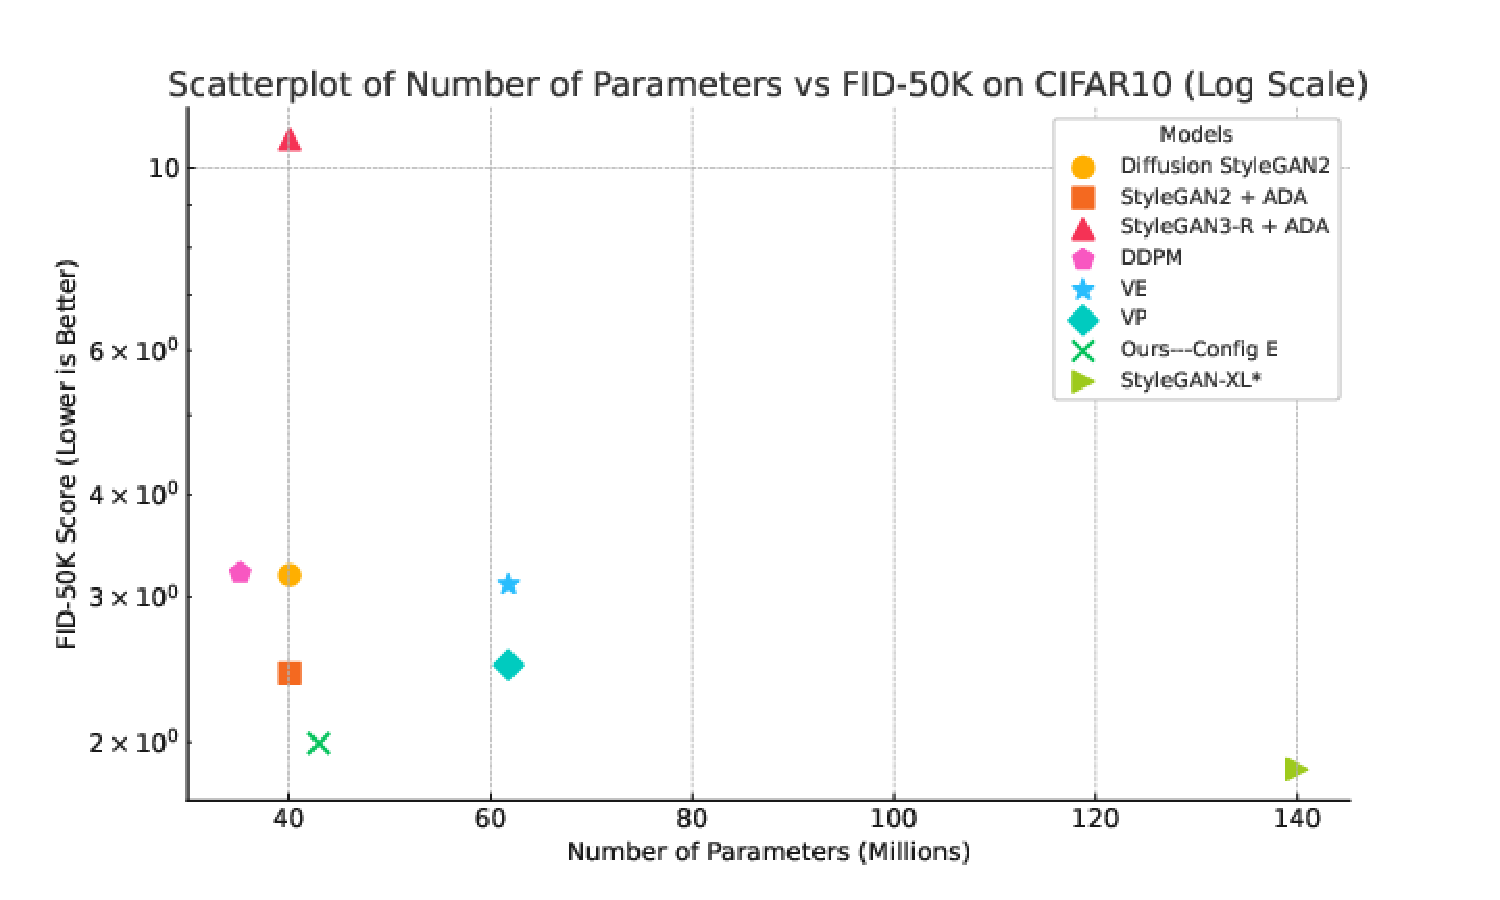
\includegraphics[width=\linewidth,clip,trim={0 0 0 2cm}]{figures/Scatterplot-FID-Parameters-CIFAR10.pdf}
    \caption{Millions of parameters vs.~FID-50K (log scale) on CIFAR-10. Lower is better.}
    \label{fig:fid-50k-vs-params-cifar-10}
\end{wrapfigure}

Many state-of-the-art GANs are derived from Projected GAN~\cite{sauer2021projected}, including StyleGAN-XL~\cite{sgxl} and the concurrent work of StyleSAN-XL~\cite{takida2024san}. These methods use a pre-trained ImageNet classifier in the discriminator. Prior work has shown that a pre-trained ImageNet discriminator can leak ImageNet features into the model~\cite{kynkaanniemi2022role}, causing the model to perform better when evaluating on FID since it relies on a pre-trained ImageNet classifier for the loss. But, this does not improve results in perceptual studies~\cite{kynkaanniemi2022role}. Our model produces its low FID without any ImageNet pre-training.

%\jt{Missing citations here for such methods.}


%\aaron{add NFEs}
%\jt{Which models in our evaluation use this? Any?}

%\jt{What is the second caveat?}

\subsection{FID --- ImageNet-32~\cite{chrabaszcz2017downsampled}}
\label{sec:imagenet32-fid-explain}
We train Config E model until convergence and with optimized hyperparameters and training schedule on ImageNet-32 (conditional generation). We compare against recent GAN models and recent diffusion models in Table~\ref{tab:imagenet32}.
We adjust the number of parameters in the generator of our model to match StyleGAN-XL~\cite{sgxl}'s generator (84M parameters). Specifically, we make the model significantly wider to match. Our method achieves comparable FID despite using a 60\% smaller discriminator (Tab.~\ref{tab:imagenet32}) and despite not using a pre-trained ImageNet classifier.
%, which has been shown to improve FID performance, but not improve results in perceptual studies~\cite{kynkaanniemi2022role}.

\vspace{-0.1cm}
\subsection{FID --- ImageNet-64~\cite{chrabaszcz2017downsampled}}
We evaluate our model on ImageNet-64 to test its scalability. We stack another resolution stage on our ImageNet-32 model, resulting in a generator of 104\ M parameters. This model is nearly 3$\times$ smaller than diffusion-like models~\cite{adm,edm,cm,icm} that rely on the ADM backbone, which contains about 300\ M parameters. Despite the smaller model size and that our model generates samples in one step, it outperforms larger diffusion models with many NFEs on FID (Tab.~\ref{tab:imagenet64}).

\vspace{-0.1cm}
\subsection{Recall}
We evaluate the recall~\cite{precrecall} of our model on each dataset to quantify sample diversity. In general, our model achieves a recall that is similar to or marginally worse than the diffusion model counterpart, yet superior to existing GAN models. For CIFAR-10, the recall of our model peaked at 0.57; as a point of comparison, StyleGAN-XL~\cite{sgxl} has a worse recall of 0.47 despite its lower FID. For FFHQ, we obtain a recall of 0.53 at 64$\times$64 and 0.49 at 256$\times$256, whereas StyleGAN2~\cite{sg2} achieved a recall of 0.43 on FFHQ-256. Our ImageNet-32 model achieved a recall of 0.63; comparable to ADM~\cite{adm}. Our ImageNet-64 model achieved recall 0.59. While this is slightly worse than $\approx$0.63 that many diffusion models achieve, it is better than BigGAN-deep~\cite{biggan} which achieved a recall of 0.48.

\begin{figure}
    \begin{floatrow}
        \capbtabbox{%
        \centering
        \resizebox{0.9\linewidth}{!}{
        \begin{tblr}{
          column{2} = {r},
          column{3} = {r},
          cell{8}{1} = {c=3}{},
          hline{2,7-8} = {-}{},
        }
    Model                                                       & NFE$\downarrow$  & FID$\downarrow$                        \\ 
    DDPM++~\cite{kim2021soft}                  & 1000 & 8.42                                   \\
    VDM~\cite{kingma2021variational}           & 1000 & 7.41                                   \\
    MSGAN~\cite{karnewar2020msg,ning2023input} & 1    & 12.3                                   \\
    ADM~\cite{adm}                             & 1000 & 3.60                                   \\
    DDPM-IP~\cite{ning2023input}               & 1000 & 2.87                                   \\
    Ours—Config E               & 1    & 1.27   \\
    \textit{With ImageNet feature leakage~\cite{kynkaanniemi2022role}:}    \\
    StyleGAN-XL*~\cite{sgxl}                   & 1    & 1.10                                  
    \end{tblr}
        }
    }{%
        \caption{\label{tab:imagenet32}ImageNet-32.}
        % \jt{some are conditional still}}
    }
    %
    \capbtabbox{
        \centering
        \resizebox{0.9\linewidth}{!}{
        \begin{tblr}{
          column{2} = {r},
          column{3} = {r},
          cell{1}{2} = {c},
          cell{1}{3} = {c},
          cell{12}{1} = {c=3}{},
          hline{2-3,11-12} = {-}{},
        }
        Model         & NFE$\downarrow$ & FID$\downarrow$ \\
        BigGAN-deep~\cite{biggan}\phantom{xx}   & 1               & 4.06            \\
        DDPM~\cite{ddpm}          & 250             & 11.0            \\
        DDIM~\cite{ddim}          & 50              & 13.7            \\
        ADM~\cite{adm}           & $^\S$250             & 2.91            \\
        EDM~\cite{edm}           & 79              & 2.23            \\
        CT~\cite{cm}            & 2               & 11.1            \\
        CD~\cite{cm}            & 3               & 4.32            \\
        iCT-deep~\cite{icm}      & 2               & 2.77            \\
        DMD~\cite{dmd}           & 1               & 2.62            \\
        Ours—Config E & 1               & 2.09            \\
        \emph{With ImageNet feature leakage~\cite{kynkaanniemi2022role}:}          &                 &                 \\
        StyleGAN-XL*~\cite{sgxl}   & 1               & 1.52            
        \end{tblr}
        }
    }
    {
        \caption{\label{tab:imagenet64}ImageNet-64.\hspace{-0.1cm} {\small \S:\hspace{-0.05cm}deterministic sampling.}}
    }
    \end{floatrow}
    \vspace{-0.25cm}
\end{figure}


% \begin{table}[ht]
%     \centering
%     \begin{tabular}{lcccccccc}
%         \toprule
%         \textbf{Model} & \textbf{\# Param.} & \textbf{IS $\uparrow$} & \textbf{FID $\downarrow$} & \textbf{Precision $\uparrow$} & \textbf{Recall $\uparrow$} & \textbf{Density $\uparrow$} & \textbf{Coverage $\uparrow$} & \textbf{Inf. (s)} \\
%         \midrule
%         ReACGAN + DiffAug (Ours) [10] & 9.4M & 10.15 & 2.64 & 0.75 & 0.65 & 0.98 & 0.90 & 0.009 \\
%         StyleGAN2-ADA [85] & 20.2M & 10.31 & 2.41 & 0.74 & 0.68 & 1.02 & 0.92 & 0.008 \\
%         StyleGAN2-ADA (Ours) [85] & 20.2M & \textbf{10.53} & 2.31 & 0.75 & 0.69 & 1.04 & 0.93 & 0.008 \\
%         StyleGAN2 + DiffAug + D2D-CE (Ours) [10] & 20.2M & 10.46 & 2.30 & 0.76 & 0.68 & 1.03 & 0.93 & 0.007 \\
%         DDPM [43] & 35.2M & 9.73 & 3.23 & 0.78 & 0.67 & 1.10 & 0.93 & 15.422 \\
%         DDPM++ [44] & 106.6M & 9.90 & 2.49 & 0.78 & 0.69 & 1.12 & 0.94 & 46.697 \\
%         NCSN++ [44] & 107.6M & 10.08 & 2.27 & 0.77 & 0.70 & 1.07 & 0.94 & 99.304 \\
%         LSGM [45] & - & 10.04 & 2.80 & 0.80 & 0.70 & 1.15 & 0.95 & - \\
%         LSGM-ODE [45] & - & 10.07 & \textbf{2.09} & 0.77 & 0.71 & 1.03 & 0.94 & - \\
%         CLD-SGM [47] & - & 9.88 & 2.38 & 0.78 & 0.69 & 1.12 & 0.94 & - \\
%         StyleGAN-XL~ & 18.0M & \textbf{11.03} & \textbf{1.88} & 0.77 & 0.59 & 1.08 & 0.94 & 0.010 \\
%         % BaselineGAN & %10.284011840820312
%         % 10.28
%         % & %1.9925376117527978 
%         % 1.99 & % 0.6899600028991699 
%         % 0.69 &&
%         \bottomrule
%     \end{tabular}
%     \caption{Comparison of various models on CIFAR10 dataset. TODO fix citation}
% \label{tab:cifar10_comparison}
%\end{table}

% \jt{Is the below meant to be a conclusion? Some of these statements are unfounded in the evidence we present so far.}
% \begin{enumerate}

%     \item We demonstrate the ability of our method to recover all modes of training data on Stacked Mnist~\ref{tab:stackedmnist}.
%     \item We beat all methods that do not use bCR (shown to overfit for FFHQ-256~\cite{}) and methods that do not leak imagenet features from a pretrained discriminator~\cite{kynkaanniemi2022role}. If we exclude these two categories of models, we are SOTA across all open source GANs. We also SOTA on a per parameter count basis on multiple GANs.
%     \item We demonstrate SOTA performance on CIFAR-10 image generation at our current parameter count, outperforming all previous GANs except for StyleGAN-XL derived ones with X\% percent of the parameters of these methods. We also do not leak features from ImageNet or use a pretrained discriminator.~\ref{tab:cifar10}. 
%     \item We achieve near SOTA on FFHQ 256 and achieve SOTA for a GAN method without bCR or feature leakage.
%     \item We achieve near state of the art results on Imagenet and achieve Pareto frontier results for total GAN model parameter size.
% \end{enumerate}
% \begin{table}[h]
\centering
\caption{FID on ImageNet-32}
\begin{tabular}{ l c c }
\toprule
Model & \textbf{Year} & FID$\downarrow$ \\
\midrule
% %Real NVP (Dinh et al.) & 2016 & 4.28 \\
% %Glow (Kingma and Dhariwal) & 2018 & 4.09 \\
% %MintNet & 2019 & 4.06 \\
% % Residual Flow & 2019 & 4.01 \\
% % BIVA Maaloe et al. & 2019 & 3.96 \\
% % ANF Huang et al. & 2020 & 3.92 \\
% % NVAE w/ flow & 2020 & 3.92 \\
% % PixelRNN & 2016 & 3.86 \\
% % Flow++ & 2019 & 3.86 \\
% % SPN Menick and Kalchbrenner & 2018 & 3.85 \\
% % Gated PixelCNN & 2016 & 3.83 \\
% % Very Deep VAE & 2020 & 3.8 \\
% % MRCNF & 2021 & 3.77 \\
% % $\delta$-VAE & 2019 & 3.77 \\
% Image Transformer~\cite{parmar2018image} & 2018 & 3.77 \\
% ScoreFlow & 2021 & 3.76 \\
% Reflected Diffusion & 2023 & 3.74 \\
% %Hourglass & 2021 & 3.74 \\
% DenseFlow-74-10 & 2021 & 3.63 \\
% i-DODE & 2023 & 3.43 \\
% MSGAN~\cite{karnewar2020msg} & 2019 & 12.3 \\
% DDPM-IP & 2023 & 2.66 \\
MSGAN~\cite{karnewar2020msg} & 2019 & 12.3 \\
VDM~\cite{kingma2021variational} & 2021 & 7.41 \\
DDPM++~\cite{kim2021soft} & 2021 & 8.42 \\
DDPM-IP~\cite{ning2023input} & 2023 & 2.87 \\
\textbf{Ours} & 2024 & 1.28 \\
StyleGAN-XL~\cite{sauer2022stylegan} & 2022 & \textbf{1.10} \\
\bottomrule
\end{tabular}
\end{table}

% \begin{table}[tO]
%     \centering
%     \begin{tabular}{c|c|c|c}
%          & FID\_50k & Precision & Recall \\
%         StyleGAN &  \\
%         StyleGAN-XL? &
%         Lots of other baselines
%     \end{tabular}
%     \caption{Caption}
%     \label{tab:my_label}
% \end{table}
% \label{sec:exp}
% % cifar10, ffhq, imagenet

% \begin{table}
%     \centering
%     %\caption{Results for CIFAR-10 generation. \aaron{add NFEs}}
%     %\vspace{-2mm}
%     \begin{tblr}{
%       column{2} = {r},
%       cell{1}{2} = {c},
%       hline{2,9,13} = {-}{},
%     }
%     Model               & FID$\downarrow$           \\
%     BigGAN~\cite{biggan}              & 14.73         \\
%     TransGAN~\cite{trans}            & 9.26          \\
%     ViTGAN~\cite{vitgan}              & 6.66          \\
%     DDGAN~\cite{ddgan}               & 3.75          \\
%     Diffusion StyleGAN2 & 3.19          \\
%     StyleGAN2 + ADA     & 2.42          \\
%     StyleGAN3-R + ADA   & 10.83         \\
%     DDPM                & 3.21          \\
%     DDIM                & 4.67          \\
%     VE                  & 3.11          \\
%     VP                  & 2.48          \\
%     Ours---Config E     & \textbf{1.99} 
%     \end{tblr}
%     %\label{tab:cifar10}
%     \caption{Results for CIFAR-10 generation. \aaron{add NFEs}}
%     \label{tab:cifar10}
% \end{table}



%%%%%%%%%%%%%%%%%%%%%%%%%%%%%%%%%%%%%%%%%%%%%%%%%%%%%%%%%%%%%
% Qualitative figures
%%%%%%%%%%%%%%%%%%%%%%%%%%%%%%%%%%%%%%%%%%%%%%%%%%%%%%%%%%%%%

% Variable to control the size of each image
% \begin{figure}
%     \centering
%     \includegraphics{example-image-a}
%     \caption{stacked mnist (qualitative figure) (from powerpoint)}
%     \label{fig:stacked-mnist}
% \end{figure}
% cifar10, ffhq, imagenet

% \noindent\begin{minipage}{.33\textwidth}
% \centering
% \captionof{table}{1000-mode coverage on StackedMNIST.}
% \vspace{-2mm}
% \begin{tblr}{
%   cell{2}{2} = {c},
%   cell{2}{3} = {c},
%   cell{3}{2} = {c},
%   cell{3}{3} = {c},
%   cell{4}{2} = {c},
%   cell{4}{3} = {c},
%   cell{5}{2} = {c},
%   cell{5}{3} = {c},
%   cell{6}{2} = {c},
%   cell{6}{3} = {c},
%   cell{7}{2} = {c},
%   cell{7}{3} = {c},
%   cell{8}{2} = {c},
%   cell{8}{3} = {c},
%   cell{9}{2} = {c},
%   cell{9}{3} = {c},
%   cell{10}{2} = {c},
%   cell{10}{3} = {c},
%   cell{11}{2} = {c},
%   cell{11}{3} = {c},
%   hline{2,11} = {1-3}{},
% }
% Model     & Modes$\uparrow$ & KLD$\downarrow$            &  \\
% DCGAN     & 99            & 3.40\phantom{0}&  \\f
% VEEGAN    & 150           & 2.95\phantom{0}&  \\
% WGAN-GP   & 959           & 0.73\phantom{0}&  \\
% PacGAN    & 992           & 0.28\phantom{0}&  \\
% StyleGAN2 & 940           & 0.42\phantom{0}&  \\
% PresGAN   & \textbf{1000} & 0.12\phantom{0}&  \\
% Adv. DSM  & \textbf{1000} & 1.49\phantom{0}&  \\
% VAEBM     & \textbf{1000} & 0.087          &  \\
% DDGAN     & \textbf{1000} & 0.071          &  \\
% Ours      & \textbf{1000} & \textbf{???} &  
% \end{tblr}
% \label{tab:stackedmnist}
% \end{minipage}%
% \begin{minipage}{.33\textwidth}
% \centering
% \captionof{table}{Results for CIFAR-10 generation.}
% \vspace{-2mm}
% \begin{tblr}{
%   column{2} = {r},
%   cell{1}{2} = {c},
%   hline{2,9,13} = {-}{},
% }
% Model               & FID$\downarrow$           \\
% BigGAN              & 14.73         \\
% TransGAN            & 9.26          \\
% ViTGAN              & 6.66          \\
% DDGAN               & 3.75          \\
% Diffusion StyleGAN2 & 3.19          \\
% StyleGAN2 + ADA     & 2.42          \\
% StyleGAN3-R + ADA   & 10.83         \\
% DDPM                & 3.21          \\
% DDIM                & 4.67          \\
% VE                  & 3.11          \\
% VP                  & 2.48          \\
% Ours                & \textbf{1.99} 
% \end{tblr}
% \label{tab:cifar10}
% \end{minipage}%
% \begin{minipage}{.33\textwidth}
% \centering
% \captionof{table}{Results on FFHQ ($256\times256$).}
% \vspace{-2mm}
% \begin{tblr}{
%   column{2} = {r},
%   cell{1}{2} = {c},
%   hline{2,5} = {-}{},
%   hline{2,9} = {-}{},
% }
% Model       & FID$\downarrow$  \\
% StyleGAN2   & 3.78 \\
% StyleGAN3-T & 4.81 \\
% StyleGAN3-R & 3.92 \\
% LDM & 4.98\\
% ADM (DDIM) & 8.41\\
% ADM (DPM-Solver) & 8.40\\
% Diffusion Autoencoder & 5.81\\
% Ours        & \textbf{2.95} 
% \end{tblr}
% \label{tab:ffhq256}
% \end{minipage}


% \input{tables/cifar10}
% \input{tables/ffhq256}
% \input{tables/MNIST}
\begin{figure}[h!]
    \newlength{\imgsize}
    \setlength{\imgsize}{0.10\linewidth} % Adjust this value to change the size of the images
    
    % New command to include images from a specific directory
    \newcommand{\qualitativeimg}[1]{%
        \includegraphics[width=\imgsize]{figures/qualitative/ffhq-256-000139623/image-#1.jpg}%
    }
    
    \setlength{\tabcolsep}{0pt} % Remove spacing between columns
    \renewcommand{\arraystretch}{0} % Remove spacing between rows
    
    \centering
    \begin{tabular}{cccccccc} % Eight columns
        \qualitativeimg{64} & \qualitativeimg{65} & \qualitativeimg{66} & \qualitativeimg{67} & \qualitativeimg{128} & \qualitativeimg{69} & \qualitativeimg{70} & \qualitativeimg{71} \\
        \qualitativeimg{72} & \qualitativeimg{73} & \qualitativeimg{74} & \qualitativeimg{75} & \qualitativeimg{76} & \qualitativeimg{77} & \qualitativeimg{78} & \qualitativeimg{79} \\
        \qualitativeimg{80} & \qualitativeimg{81} & \qualitativeimg{82} & \qualitativeimg{83} & \qualitativeimg{84} & \qualitativeimg{85} & \qualitativeimg{86} & \qualitativeimg{87} \\
        \qualitativeimg{88} & \qualitativeimg{89} & \qualitativeimg{90} & \qualitativeimg{91} & \qualitativeimg{92} & \qualitativeimg{93} & \qualitativeimg{94} & \qualitativeimg{95} \\
        \qualitativeimg{96} & \qualitativeimg{97} & \qualitativeimg{98} & \qualitativeimg{99} & \qualitativeimg{100} & \qualitativeimg{101} & \qualitativeimg{102} & \qualitativeimg{103} \\
        \qualitativeimg{104} & \qualitativeimg{105} & \qualitativeimg{106} & \qualitativeimg{107} & \qualitativeimg{108} & \qualitativeimg{109} & \qualitativeimg{110} & \qualitativeimg{111} \\
        \qualitativeimg{112} & \qualitativeimg{113} & \qualitativeimg{114} & \qualitativeimg{115} & \qualitativeimg{116} & \qualitativeimg{117} & \qualitativeimg{118} & \qualitativeimg{119} \\
        \qualitativeimg{120} & \qualitativeimg{121} & \qualitativeimg{122} & \qualitativeimg{123} & \qualitativeimg{124} & \qualitativeimg{125} & \qualitativeimg{126} & \qualitativeimg{127} \\
    \end{tabular}
    \caption{Qualitative examples of sample generation from our Config E on FFHQ-256.}
    \label{fig:ffhq-256-teaser}
\end{figure}


\section{Discussion}
\label{sec:discussion}

We discuss related work, limitations, and some future directions.

\paragraph{Related Work.}
\cref{sec:discussion:selection} discusses how the selection mechanism relates to similar concepts.
\cref{sec:related} has an extended related work of SSMs and other related models.

\paragraph{No Free Lunch: Continuous-Discrete Spectrum.}
Structured SSMs were originally defined as discretizations of continuous systems \eqref{eq:ssm},
and have had a strong inductive bias toward continuous-time data modalities such as perceptual signals (e.g.\ audio, video).
As discussed in \cref{sec:method:motivation,sec:method:properties}, the selection mechanism overcomes their weaknesses
on discrete modalities such as text and DNA;
but this conversely can impede their performance on data that LTI SSMs excel on.
Our ablations on audio waveforms examine this tradeoff in more detail.

\paragraph{Downstream Affordances.}
Transformer-based foundation models (particularly LLMs) have a rich ecosystem of properties and modes of interaction with pretrained models,
such as fine-tuning, adaptation, prompting, in-context learning, instruction tuning, RLHF, quantization, and so on.
We are particularly interested in whether Transformer alternatives such as SSMs have similar properties and affordances.

%

\paragraph{Scaling.}
Our empirical evaluation is limited to small model sizes,
below the threshold of most strong open source LLMs (e.g. Llama \citep{touvron2023llama})
as well as other recurrent models such as RWKV~\citep{peng2023rwkv} and RetNet~\citep{sun2023retentive},
which have been evaluated at the 7B parameter scale and beyond.
It remains to assess whether Mamba still compares favorably at these larger sizes.
We also note that scaling SSMs may involve further engineering challenges and adjustments to the model
that are not discussed in this paper.

%


\iftoggle{arxiv}{
\subsubsection*{Acknowledgments}

We are grateful to the NVIDIA CUTLASS team (especially Haicheng Wu, Aniket
Shivam, and Cris Cecka) for helping us understand Hopper's
programming model and for their library, which provides clean and powerful building blocks for the implementation of \fat.
We thank the cuDNN team for the idea of in-kernel transpose for FP8.
The idea of overlapping GEMMs and softmax was inspired by insightful
conversations with Christopher R{\'e}, Benjamin Spector, Aniket Shivam, and Markus Hoehnerbach.
The pingpong scheduling is adapted from the warp-specialized pingpong GEMM
implementation in CUTLASS.
We appreciate Driss Guessous for integrating \fa to PyTorch.
\fat has benefited from helpful discussions with Horace He on different attention
variants, with Hao Liu and Phil Wang on distributed attention, and with Daniel
Haziza and Chris De Sa on quantization.
We thank Meta, Together AI, and Princeton Language and Intelligence (PLI) for compute support.

}{}

\bibliography{ref}
\bibliographystyle{plainnat}

\newpage
\appendix
%
\section{Related Work}
%


\subsection{Classical Approaches} \label{appendix:related_work_classical}

Classical approaches in time series modeling include the Box-Jenkins method \citep{box1968some}, exponential smoothing  \citep{hyndman2008forecasting, winters1960forecasting}, autoregressive integrated moving average (ARIMA) \citep{box1970time}, and state-space models \citep{hamilton1994state}. In such approaches, the model is usually manually selected based analyzing time series features (e.g., seasonality and order of non-stationarity), where the selected model is then fitted for each individual time series. While classical approaches may be more interpretable than recent deep learning techniques, the domain expertise and manual labor needed to succesfully apply them renders them infeasible to the common setting of modeling thousands, or millions, of time series.

\subsection{Deep Learning Approaches} \label{appendix:related_work_deep}

% (Deep AR, LSTMs, RNNs)
\textbf{Recurrent models.}  Common deep learning architectures for modeling sequence data are the family of recurrent neural networks, which include GRUs~\citep{chung2014empirical}, LSTMs~\citep{hochreiter1997long}, and DeepAR \citep{salinas2020deepar}. However, due to the recurrent nature of RNNs, they are slow to train and may suffer from vanishing/exploding gradients, making them difficult to train \citep{pascanu2013difficulty}. \\

\textbf{Deep State Space models.} Recent work has investigated combining the expressive strengths of SSMs with the scalable strengths of deep neural networks \citep{rangapuram2018, gu2021efficiently}. \cite{rangapuram2018} propose to train a global RNN that transforms input covariates to sequence-spcific SSM parameters; however, one downside of this approach is that they inherit the drawbacks of RNNs. More recent approaches, such as LSSL \citep{gu2021combining}, S4 \citep{gu2021efficiently}, S4D \citep{gu2022parameterization}, and S5 \citep{smith2022simplified}, directly parameterize the layers of a neural network with multiple linear SSMs, and overcome common recurrent training drawbacks by leveraging the convolutional view of SSMs. While deep SSM models have been shown great promise in time series modeling, we show in our work -- which builds off deep SSMs -- that current deep SSM approaches are not able to capture autoregressive processes due to their continuous nature.  \\


\textbf{Neural differential equations as nonlinear state spaces.}
%
\citep{chen2018neural} parametrizes the vector field of continuous--time autonomous systems. These models, termed \textit{Neural Differential Equations} (NDEs) have seen extensive application to time series and sequences, first by \cite{rubanova2019latent} and then by \cite{kidger2020neural,morrill2021neural,massaroli2021differentiable} with the notable extension to \textit{Neural Controlled Differential Equations} (Neural CDEs). Neural CDEs can be considered the continuous--time, nonlinear version of state space models and RNNs \citep{kidger2022neural}. Rather than introducing nonlinearity between linear state space layers, Neural CDEs model nonlinear systems driven by a control input. 

The NDE framework has been further applied by \cite{poli2019graph} to model graph time series via \textit{Neural Graph Differential Equations}. In \cite{queiruga2020continuous}, a continuous-depth ResNet generalization based on ODEs is proposed, and in \cite{kim2021stiff} numerical techniques to enable learning of stiff dynamical systems with Neural ODEs are investigated. The idea of parameterizing the vector field of a differential equation with a neural network, popularized by NDEs, can be traced back to earlier works \citep{funahashi1993approximation, zhang2014comprehensive, weinan2017proposal}. \\



\textbf{Transformers.} 
While RNNs and its variants have shown some success at time series modeling, a major limitation is their applicability to long input sequences. Since RNNs are recurrent by nature, they require long traversal paths to access past inputs, which leads to vanishing/exploding gradients and as a result struggle with capturing long-range dependencies. 

To counteract the long-range dependency problem with RNNs, a recent line of work considers Transformers for time series modeling. The motivation is that due to the attention mechanism, a Transformer can directly model dependencies between any two points in the input sequence, independently of how far apart the points are. However, the high expressivity of the attention mechanism comes at the cost of the time and space complexity being quadratic in sequence length, making Transformers infeasible for very long sequences. As a result, many works consider specialized Transformer architectures with sparse attention mechanisms to bring down the quadratic complexity. For example, \cite{beltagy2020longformer} propose LogSparse self-attention, where a cell attends to a subset of past cells (as opposed to all cells), where closer cells are attended to more frequently, proportional to the log of their distance, which brings down complexity from $\mathcal{O}(\ell^2)$ to $\mathcal{O}(\ell(\log \ell)^2)$. \cite{zhou2021informer} propose ProbSparse self-attention, which achieves $\mathcal{O}(\ell \log \ell)$ time and memory complexity, where they propose a generative style decoder to speed inference. \cite{liu2022pyraformer} propose a pyramidal attention mechanism which shows linear time and space complexity with sequence length. Autoformer \citep{wu2021autoformer} suggests more specialization is needed in time series with a decomposition forecasting architecture, which extracts long-term stationary trend from the seasonal series and utilizes an auto-correlation mechanism, which discovers the period-based dependencies. \cite{zhou2022fedformer} believes previous attempts of Transformer-based architectures do not capture global statistical properties, and to do so requires an attention mechanism in the frequency domain. Confromer \citep{gulati2020conformer} stacks convolutional and self-attention modules into a shared layer to combine the strengths of local interactions from convolutional modules and global interactions from self-attention modules. Perceiver AR \citep{hawthorne2022general} builds on the Perceiver architecture, which reduces the computational complexity of transformers by performing self-attention in a latent space, and extends Perceiver's applicability to causal autoregressive generation.

While these works have shown exciting progress on time series forecasting, their proposed architectures are specialized to handle specific time series settings (e.g., long input sequences, or seasonal sequences), and are commonly trained to output a fixed target horizon length \citep{zhou2021informer}, \ie{} as \emph{direct multi-step forecasting} (DMS) \cite{https://doi.org/10.1111/j.1467-6419.2007.00518.x}. Thus, while effective at specific forecasting tasks, their setups are not obviously applicable to a broad range of time series settings (such as forecasting arbitrary horizon lengths, or generalizing to classification or regression tasks).
%

Moreover, \cite{zeng2022transformers} showed that simpler alternatives to Transformers, such as data normalization plus a single linear layer (NLinear), can outperform these specialized Transformer architectures when similarly trained to predict the entire fixed forecasting horizons. Their results suggest that neither the attention mechanism nor the proposed modifications of these time series Transformers may be best suited for time series modeling. Instead, the success of these prior works  may just be from learning to forecast the entire horizon with fully connected dependencies between prior time-step inputs and future time-step outputs, where a fully connected linear layer is sufficient. \\

\textbf{Other deep learning methods.} Other works also investigate pure deep learning architectures with no explicit temporal components, and show these models can also perform well on time series forecasting. \cite{oreshkin2019n} propose N-BEATS, a deep architecture based on backward and forward residual links. Even simpler, \cite{zeng2022transformers} investigate single linear layer models for time series forecasting. Both works show that simple architectures are capable of achieving high performance for time series forecasting. In particular, with just data normalization, the NLinear model in \cite{zeng2022transformers} obtained state-of-the-art performance on the popular Informer benchmark~\cite{zhou2021informer}. Given an input sequence of past lag terms and a target output sequence of future horizon terms, for every horizon output their model simply learns the fully connected dependencies between that output and every input lag sample. However, FCNs such as NLinear also carry inefficient downsides. Unlike Transformers and SSM-based models, the number of parameters for FCNs scales directly with input and output sequence length, \ie{} $\mathcal{O}(\ell h)$ for $\ell$ inputs and $h$ outputs. Meanwhile, \ourmethod{} shows that the SSM can improve the modeling quality of deep architectures, while maintaining constant parameter count regardless of input or output length. Especially when forecasting long horizons, we achieve higher forecasting accuracy with smaller models.

% \header{S4}\\
\section{Addition Details on Algorithms}

\subsection{Asynchrony Through Warp Specialization for the Backward Pass}
\label{sec:algo_ws_bwd}

Similar to the forward pass~\cref{sec:algo_ws}, we use warp specialization to
handle asynchrony.
Instead of just a simple producer-consumer pattern in the forward pass, we add
one extra role of a $\vdQ$ writer, since we need to accumulate the value of $\vdQ$
produced by each thread block to the global value of $\vdQ$.
This $\vdQ$ accumulation introduces memory contention (many thread blocks writing to the same
location) so having a separate warp to handle this (along with asynchrony) will
avoid blocking the rest of the warps in the thread block to perform the next
computation (matmul).

We include the backward pass with warp specialization in~\cref{alg:flash3_wgmma_ws_bwd}.
\begin{algorithm}[H]
    \caption{\small\label{alg:flash3_wgmma_ws_bwd}\fat backward pass with warp specialization}
    \begin{algorithmic}[1]
\REQUIRE Matrices $\vQ, \vK, \vV, \vO, \vdO \in \mathbb{R}^{N \times d}$ in HBM,
logsumexp vector $L \in \mathbb{R}^N$ in HBM, block sizes $B_c$, $B_r$.
\STATE In a preprocessing kernel, compute $D = \mathrm{rowsum}(\vdO \circ \vO) \in \mathbb{R}^d$ (pointwise multiply), write
$D$ to HBM and divide it into $T_r$ blocks $D_1, \dots, D_{T_r}$ of size
$B_r$ each.
\STATE Divide $\vQ$ into $T_r = \left\lceil\frac{N}{B_r} \right\rceil$ blocks $\vQ_1, \dots, \vQ_{T_r}$ of size $B_r \times d$ each,
and divide $\vK, \vV$ in to $T_c = \left\lceil \frac{N}{B_c} \right\rceil$ blocks $\vK_1, \dots, \vK_{T_c}$ and
$\vV_1, \dots, \vV_{T_c}$, of size $B_c \times d$ each.
\STATE Divide $\vdO$ into $T_r$ blocks $\vdO_i, \dots, \vdO_{T_r}$
of size $B_r \times d$ each, and divide $L$ into $T_r$ blocks $L_i, \dots, L_{T_r}$ of size
$B_r$ each.
\STATE Initialize pipeline object to manage barrier synchronization with $s$-stage circular SMEM buffer.
\IF {in producer warpgroup}
\STATE Deallocate predetermined number of registers.
\STATE Issue load $\vK_j$ and $\vV_j$ from HBM to shared memory.
\STATE Upon completion, commit to notify consumer of the load of $\vK_j$ and $\vV_j$.
\FOR{$1 \le i \leq T_r$}
    \STATE Wait for the $(i\,\%\,s)$th stage of the buffer to be consumed.
    \STATE Issue loads of $\vQ_i, \vdO_i$ from HBM to shared memory at the $(i\,\%\,s)$th stage of the buffer.
    \STATE Upon completion, commit to notify consumers of the loads of $\vQ_i, \vdO_i$.
\ENDFOR
\ELSIF {in consumer warpgroups}
\STATE Reallocate predetermined number of registers as function of number of consumer warps.
\STATE On-chip, Initialize $\vdK_j = (0)_{B_c \times d}, \vdV_j = (0)_{B_c \times d}$ .
\STATE Wait for $\vK_j$ and $\vV_j$ to be loaded in shared memory.
\FOR{$1 \le i \leq T_r$}
\STATE Wait for $\vQ_i$ to be loaded in shared memory.
\STATE Load $L_i, D_i$ from HBM to on-chip SRAM.
\STATE On chip, compute $\vS_{i}^{(j)} = \vQ_i \vK_j^T \in \mathbb{R}^{B_r \times B_c}$
(SS-GEMM). Commit.
\STATE Wait for $\vdO_i$ to be loaded in shared memory.
\STATE On chip, compute $\vdP_{i}^{(j)} = \vdO_{i} \vV_j^\top \in \mathbb{R}^{B_r \times B_c}$
(SS-GEMM). Commit.
\STATE On chip, wait for $\vS_{i}^{(j)}$, then compute $\vP_{i}^{(j)} = \exp(\vS_{ij} - L_{i}) \in \mathbb{R}^{B_r \times B_c}$.
\STATE On chip, wait for $\vdP_i^{(j)}$, then compute $\vdS_{i}^{(j)} = \vP_{i}^{(j)} \circ (\vdP_{i}^{(j)} - D_i) \in \mathbb{R}^{B_r \times B_c}$.
\STATE On chip, compute
$\vdV_j \leftarrow \vdV_j + (\vP_{i}^{(j)})^\top \vdO_i \in \mathbb{R}^{B_c \times d}$ (RS-GEMM). Commit.
\STATE On chip, compute $\vdK_{j} \leftarrow \vdK_j + {\vdS_{i}^{(j)}}^\top \vQ_i \in \mathbb{R}^{B_c \times
  d}$ (RS-GEMM). Commit and wait for both $\vdV_j$ and $\vdK_j$.
\STATE On chip, compute $\vdQ_{i}^{(\mathrm{local})} = \vdS_{i}^{(j)} \vK_j \in
\mathbb{R}^{B_r \times d}$ (SS-GEMM), and write $\vdQ_i^{(\mathrm{local})}$ to smem. Notify
the $\vdQ$-writer.
\ENDFOR
\ELSIF{in $\vdQ$-writer warp}
\FOR{$1 \le i \leq T_r$}
\STATE Wait for $\vdQ_i^{(\mathrm{local})}$ to be ready in smem.
\STATE Using a semaphore, atomically add $\vdQ_i^{(\mathrm{local})}$ to $\vdQ_i$ in global memory.
\ENDFOR
\ENDIF
\end{algorithmic}
\end{algorithm}

\subsection{2-Stage Pipelining SASS Analysis}
\label{sec:2-stage-sass}

We give simplified SASS code for the inside of the consumer warpgroup mainloop.
\begin{small}
\begin{verbatim}
// Compute row_max
FMNMX.FTZ R0, R24, R6, !PT ;
SHFL.BFLY PT, R185, R2, 0x2, 0x1f ;
… FMNMX and SHFL.BFLY … 

// Apply exp2 and row_sum. Rescale O.
FMUL.FTZ R2, R4, UR9 ;
MUFU.EX2 R185, R184 ;                                            
FFMA.FTZ R24, R24, UR9, -R6.reuse ;
FADD.FTZ R24, R211, R24 ;                              
… FMUL, FFMA, FMUL, MUFU.EX2, FADD …

// FP32 -> FP16 conversion are interleaved with exp2, row_sum and O rescaling.
F2FP.F16.F32.PACK_AB R231, R25, R231 ;
… F2FP, FMUL, MUFU, FFMA, FADD ...

// Start the first WGMMA. Broken down into 8 HGMMAs.
// The first 7 HGMMAs are packed together.
WARPGROUP.ARRIVE ;
HGMMA.64x192x16.F32 R24, gdesc[UR44], RZ, !UPT ;
... HGMMA x 6 ...

// FP32->FP16, exp2, row_sum, O rescaling are interleaved with HGMMA. 
F2FP.F16.F32.PACK_AB R214, R214, R187 ; 
MUFU.EX2 R234, R5 ;
FADD.FTZ R237, R187, R2 ;
… F2FP, MUFU, FADD …

// The last HGMMA is issued here. No need to wait.
HGMMA.64x192x16.F32 R24, gdesc[UR44], R24, gsb0 ;

// Start the second WGMMA. Broken down into 12 HGMMAs.
// All 12 HGMMAs are packed together. Not interleaved with other instructions.
WARPGROUP.ARRIVE ;
HGMMA.64x128x16.F32 R120, R228, gdesc[UR8].tnspB, R120 ;
... HGMMA x 10 ...
HGMMA.64x128x16.F32 R120, R184, gdesc[UR8].tnspB, R120, gsb0 ;

// wgmma.wait_group at the end.
WARPGROUP.DEPBAR.LE gsb0, 0x0 ; 

\end{verbatim}
\end{small}

We make the following observations:
\begin{enumerate}
    \item Softmax is reordered to the very beginning, even before the first WGMMA. \TD{why?}
    \item The first WGMMA is interleaved with softmax and FP32 $\rightarrow$ FP16 datatype conversion of $\vS$. This indicates that WGMMA and non-WGMMAs are executed in parallel.
    \item \verb|exp2|, \verb|row\_sum|, O rescaling and FP32 $\rightarrow$ FP16 conversions are interleaved together. \TD{what's the benifit since these instructions are synced?} 
    \item The second WGMMA is not overlapped with other instructions, as expected.
\end{enumerate}
Overall, SASS shows that the 2-stage pipelining idea works as expected.

\subsection{3-Stage Pipelining Algorithm}
\label{sec:3-stage}
We experiment with a 3-stage pipelining algorithm to parallelize the first WGMMA from iteration $j+2$, softmax from iteration $j+1$, and the second WGMMA from iteration $j$. We describe this algorithm in \cref{alg:flash3_3_stage_wgmma}. 
This algorithm behaves worse than the 2-stage pipelining algorithm due to the reasons below:

\begin{figure}[ht]
    \centering
    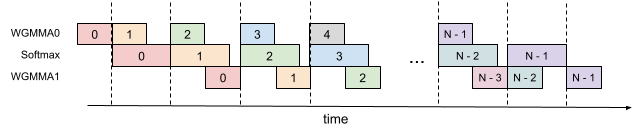
\includegraphics[width=.95\linewidth]{figs/3_stage_pipelining.png}
    \caption{3-Stage Pipelining}
    \label{fig:3_stage_pipelining}
\end{figure}

\begin{algorithm}[H]
    \caption{\small\label{alg:flash3_3_stage_wgmma}\sysnameone 3-stage pipelining consumer warpgroup forward pass}
    \begin{algorithmic}[1]
      \REQUIRE Matrices $\vQ, \vK, \vV \in \mathbb{R}^{N \times d}$ in HBM, block sizes $B_c$, $B_r$.
      Each warpgroup reads 1 block Qi of size $B_r \times d$, $T_c = \left\lceil \frac{N}{B_c} \right\rceil$ blocks $\vK_1, \dots, \vK_{T_c}$ and
      $\vV_1, \dots, \vV_{T_c}$ of size $B_c \times d$.
      Each warpgroup writes 1 output block $\vO_i$ of size $B_r \times d$, and 1 logsumexp block $L_i$ of size $B_r$.
      \STATE Initialization. Load $\vQ_i$ from HBM to on-chip SRAM.
      Initialize $\vO_{i}, \ell_{i}, m_{i}, scale\_o$.
      \STATE Wait for the producer warpgroup loading $\vK_0$ from HBM to on-chip SRAM.
      \STATE Compute $\vS = \vQ_i \vK_0^T$ using WGMMA. Commit and wait.
      \STATE Compute $m_{i}$, $\tilde{\vP}_{i}$, $\ell_{i}$, $scale\_o$ based on $\vS$.
      \STATE Wait for the producer warpgroup loading $\vK_1$ from HBM to on-chip SRAM.
      \STATE Compute $\vS = \vQ_i \vK_1^T$ using WGMMA. Commit and wait.
      \FOR{$2 \le j < T_c - 2$}
        \STATE Wait for the producer warpgroup loading $\vK_j$ from HBM to on-chip SRAM.
        \STATE Compute $\vS\_next = \vQ_i \vK_{j}^T$ using WGMMA. Commit but do not wait.
        \STATE Wait for the producer warpgroup loading $\vV_{j-2}$ from HBM to on-chip SRAM.
        \STATE Rescale $\vO_{i}$ based on $scale\_o$.
        \STATE Compute
        $\vO_{i} = \vO_{i} + \tilde{\vP}_{i} \vV_{j-2}$ using WGMMA. Commit but do not wait.
        \STATE Compute $m_{i}$, $\tilde{\vP}_{i}\_next$, $\ell_{i}$, $scale\_o$ based on $\vS$.
        \STATE Wait for all previous WGMMAs.
        \STATE Copy $\vS\_next$ to $\vS$.
        \STATE Copy $\tilde{\vP}_{i}\_next$ to $\tilde{\vP}_{i}$.
      \ENDFOR
      \STATE Wait for the producer warpgroup loading $\vV_{T_c-2}$ from HBM to on-chip SRAM.
      \STATE Rescale $\vO_{i}$ based on $scale\_o$.
      \STATE Compute
      $\vO_{i} = \vO_{i} + \tilde{\vP}_{i} \vV_{T_c-2}$ using WGMMA. Commit and wait.
      \STATE Compute $m_{i}$, $\tilde{\vP}_{i}$, $\ell_{i}$, $scale\_o$ based on $\vS$.
      \STATE Wait for the producer warpgroup loading $\vV_{T_c-1}$ from HBM to on-chip SRAM.
      \STATE Rescale $\vO_{i}$ based on $scale\_o$.
      \STATE Compute
      $\vO_{i} = \vO_{i} + \tilde{\vP}_{i} \vV_{T_c-1}$ using WGMMA. Commit and wait.
      \STATE Epilogue. Rescale $\vO_{i}$ based on $\ell_{i}$. Compute $L_{i}$ based on $\ell_{i}$ and $m_{i}$. Write $\vO_{i}$ and $L_{i}$ to HBM as the $i$-th block of $\vO$ and $L$.
    \end{algorithmic}
  \end{algorithm}

\paragraph{Overlapping.} 
We expected that softmax can be overlapped with (the first WGMMA + the second WGMMA). However, the compiler doesn't cooperate in this way.
SASS code shows that only the first WGMMA is overlapped with softmax, while the second WGMMA is not. It's not clear why the compiler chooses to reorder instructions in this way.

\paragraph{Register pressure.}
This algorithm requires more registers compared to the 2-stage pipelining algorithm. 
In theory, it needs to store an extra $\tilde{\vP}_{i}$ and $scale\_o$, which is of size $B_r \times B_c \times \text{sizeof}(\text{input\_data\_type}) + B_r \times \text{sizeof}(\text{float})$.
As a result, a smaller block size needs to be chosen.














\section{Addition Details on Experiments and Benchmarking}

\subsection{System and libraries}
\label{sec:system}

We benchmark the speed on an H100 80GB SXM5 (700W).
We generally use the latest versions of the libraries, at the time of writing
(May 2024).
Specifically, we use:
\begin{itemize}
\item CUDA 12.3
\item cuDNN 9.1.1.17
\item CUTLASS 3.5
\item \fa 2.5.8
\item Triton nightly 3.0.0.post20240424212437
\item PyTorch 2.3.0
\end{itemize}

To reduce variability, we fix the GPU clock speed to 1830MHz (clock speed used
to calculate the 989 TFLOPS FP16 theoretical max throughput).
We repeat the benchmarks 100 times and take the average timing.






\subsection{FP8 Attention Full Results}
\label{sec:benchmark_attn_fp8_full}

We use following sequence lengths: 512, 1024, 2048, 4224, 8448, 16896.
When sequence length $\geq$ 4k, we make it also divisible by 132 (number of SMs in H100 SXM5) to avoid wave quantization.

\begin{figure}[ht]
  \centering
  \begin{subfigure}{.5\textwidth}
    \centering
    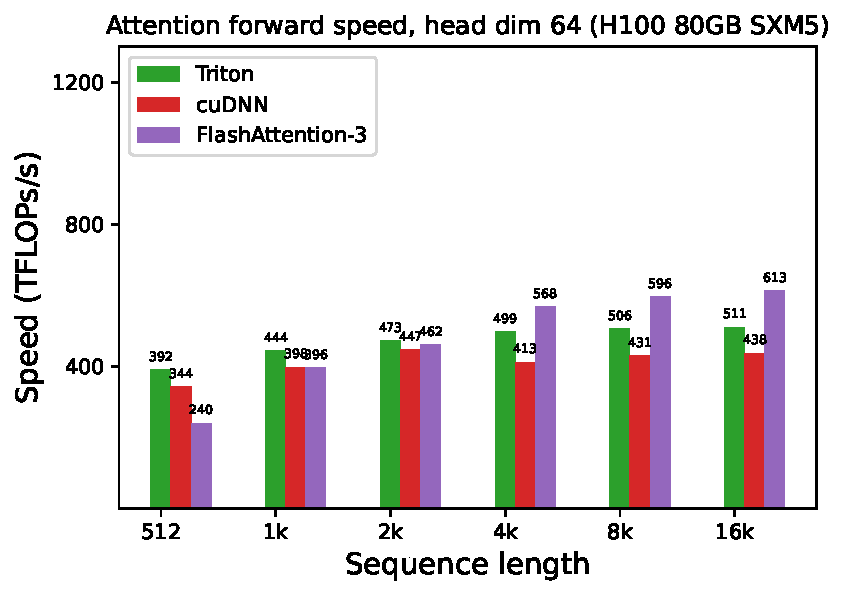
\includegraphics[width=.95\linewidth]{figs/flash3_h100_fp8_causal_False_hdim_64_fwd_speed.pdf}
    \caption{Forward, without causal mask, head dim 64}
  \end{subfigure}%
  \begin{subfigure}{.5\textwidth}
    \centering
    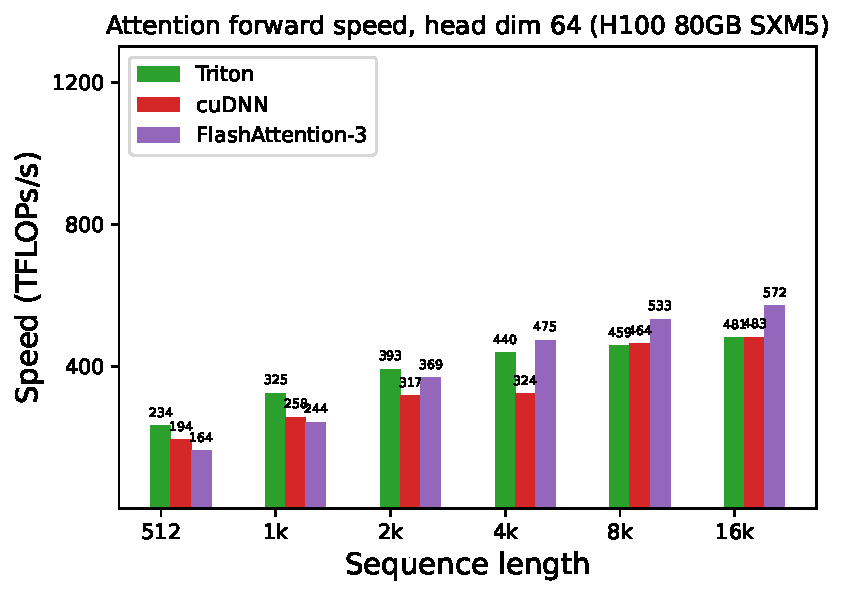
\includegraphics[width=.95\linewidth]{figs/flash3_h100_fp8_causal_True_hdim_64_fwd_speed.pdf}
    \caption{Forward, with causal mask, head dim 64}
  \end{subfigure}
  \begin{subfigure}{.5\textwidth}
    \centering
    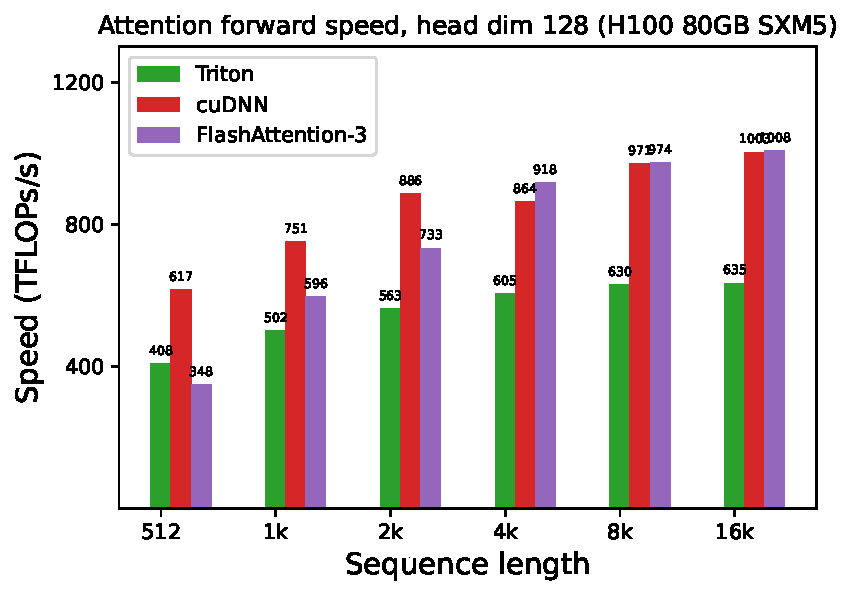
\includegraphics[width=.95\linewidth]{figs/flash3_h100_fp8_causal_False_hdim_128_fwd_speed.pdf}
    \caption{Forward, without causal mask, head dim 128}
  \end{subfigure}%
  \begin{subfigure}{.5\textwidth}
    \centering
    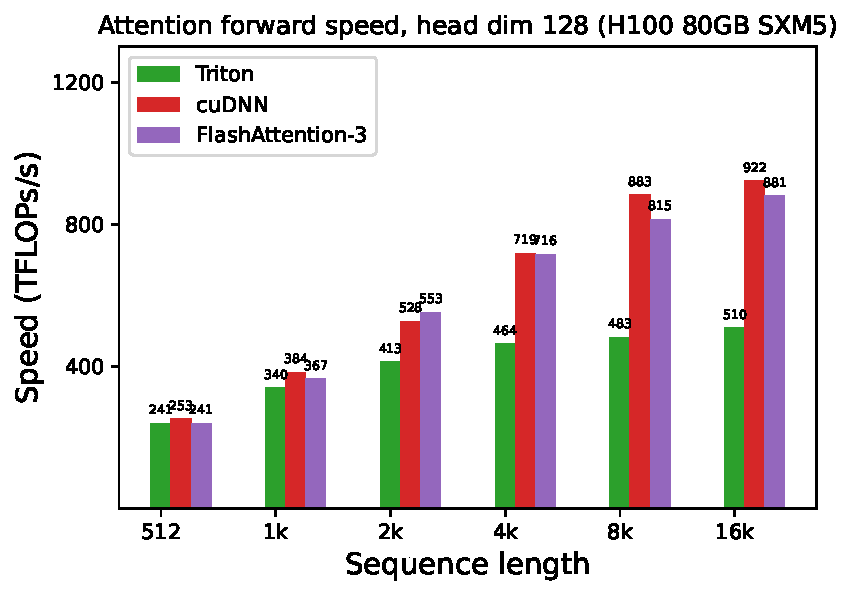
\includegraphics[width=.95\linewidth]{figs/flash3_h100_fp8_causal_True_hdim_128_fwd_speed.pdf}
    \caption{Forward, with causal mask, head dim 128}
  \end{subfigure}
  \begin{subfigure}{.5\textwidth}
    \centering
    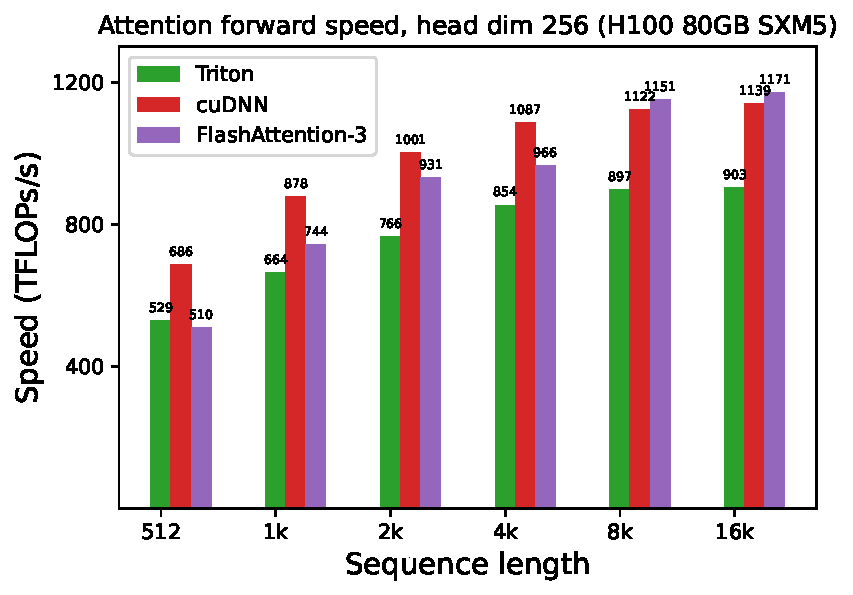
\includegraphics[width=.95\linewidth]{figs/flash3_h100_fp8_causal_False_hdim_256_fwd_speed.pdf}
    \caption{Forward, without causal mask, head dim 256}
  \end{subfigure}%
  \begin{subfigure}{.5\textwidth}
    \centering
    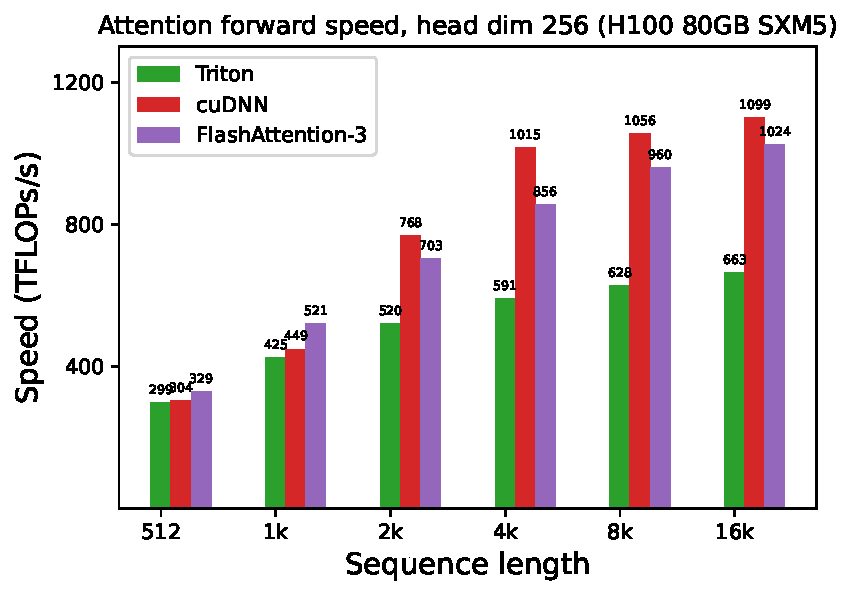
\includegraphics[width=.95\linewidth]{figs/flash3_h100_fp8_causal_True_hdim_256_fwd_speed.pdf}
    \caption{Forward, with causal mask, head dim 256}
  \end{subfigure}
  \caption{Attention forward speed (FP8) on H100 GPU}
  \label{fig:benchmark_attn_fwd_full}
\end{figure}


\iftoggle{arxiv}{}{
\pagebreak 
\section*{NeurIPS Paper Checklist}

% %%% BEGIN INSTRUCTIONS %%%
% The checklist is designed to encourage best practices for responsible machine learning research, addressing issues of reproducibility, transparency, research ethics, and societal impact. Do not remove the checklist: {\bf The papers not including the checklist will be desk rejected.} The checklist should follow the references and follow the (optional) supplemental material.  The checklist does NOT count towards the page
% limit. 

% Please read the checklist guidelines carefully for information on how to answer these questions. For each question in the checklist:
% \begin{itemize}
%     \item You should answer \answerYes{}, \answerNo{}, or \answerNA{}.
%     \item \answerNA{} means either that the question is Not Applicable for that particular paper or the relevant information is Not Available.
%     \item Please provide a short (1–2 sentence) justification right after your answer (even for NA). 
%    % \item {\bf The papers not including the checklist will be desk rejected.}
% \end{itemize}

% {\bf The checklist answers are an integral part of your paper submission.} They are visible to the reviewers, area chairs, senior area chairs, and ethics reviewers. You will be asked to also include it (after eventual revisions) with the final version of your paper, and its final version will be published with the paper.

% The reviewers of your paper will be asked to use the checklist as one of the factors in their evaluation. While "\answerYes{}" is generally preferable to "\answerNo{}", it is perfectly acceptable to answer "\answerNo{}" provided a proper justification is given (e.g., "error bars are not reported because it would be too computationally expensive" or "we were unable to find the license for the dataset we used"). In general, answering "\answerNo{}" or "\answerNA{}" is not grounds for rejection. While the questions are phrased in a binary way, we acknowledge that the true answer is often more nuanced, so please just use your best judgment and write a justification to elaborate. All supporting evidence can appear either in the main paper or the supplemental material, provided in appendix. If you answer \answerYes{} to a question, in the justification please point to the section(s) where related material for the question can be found.

% IMPORTANT, please:
% \begin{itemize}
%     \item {\bf Delete this instruction block, but keep the section heading ``NeurIPS paper checklist"},
%     \item  {\bf Keep the checklist subsection headings, questions/answers and guidelines below.}
%     \item {\bf Do not modify the questions and only use the provided macros for your answers}.
% \end{itemize} 
 

%%% END INSTRUCTIONS %%%


\begin{enumerate}

\item {\bf Claims}
    \item[] Question: Do the main claims made in the abstract and introduction accurately reflect the paper's contributions and scope?
    \item[] Answer: \answerYes{} % Replace by \answerYes{}, \answerNo{}, or \answerNA{}.
    \item[] Justification: Claim of stability is justified by Figure~\ref{fig:mnist_loss_curve} and later experimental performance. Claim of convergence properties is justified in Appendices A,B,C. Claim of SOTA GAN is experimentally justified in Section~\ref{sec:exp}. Claims are bound to specific datasets.
    \item[] Guidelines:
    \begin{itemize}
        \item The answer NA means that the abstract and introduction do not include the claims made in the paper.
        \item The abstract and/or introduction should clearly state the claims made, including the contributions made in the paper and important assumptions and limitations. A No or NA answer to this question will not be perceived well by the reviewers. 
        \item The claims made should match theoretical and experimental results, and reflect how much the results can be expected to generalize to other settings. 
        \item It is fine to include aspirational goals as motivation as long as it is clear that these goals are not attained by the paper. 
    \end{itemize}

\item {\bf Limitations}
    \item[] Question: Does the paper discuss the limitations of the work performed by the authors?
    \item[] Answer: \answerYes{} % Replace by \answerYes{}, \answerNo{}, or \answerNA{}.
    \item[] Justification: Please see Section 5.
    \item[] Guidelines:
    \begin{itemize}
        \item The answer NA means that the paper has no limitation while the answer No means that the paper has limitations, but those are not discussed in the paper. 
        \item The authors are encouraged to create a separate "Limitations" section in their paper.
        \item The paper should point out any strong assumptions and how robust the results are to violations of these assumptions (e.g., independence assumptions, noiseless settings, model well-specification, asymptotic approximations only holding locally). The authors should reflect on how these assumptions might be violated in practice and what the implications would be.
        \item The authors should reflect on the scope of the claims made, e.g., if the approach was only tested on a few datasets or with a few runs. In general, empirical results often depend on implicit assumptions, which should be articulated.
        \item The authors should reflect on the factors that influence the performance of the approach. For example, a facial recognition algorithm may perform poorly when image resolution is low or images are taken in low lighting. Or a speech-to-text system might not be used reliably to provide closed captions for online lectures because it fails to handle technical jargon.
        \item The authors should discuss the computational efficiency of the proposed algorithms and how they scale with dataset size.
        \item If applicable, the authors should discuss possible limitations of their approach to address problems of privacy and fairness.
        \item While the authors might fear that complete honesty about limitations might be used by reviewers as grounds for rejection, a worse outcome might be that reviewers discover limitations that aren't acknowledged in the paper. The authors should use their best judgment and recognize that individual actions in favor of transparency play an important role in developing norms that preserve the integrity of the community. Reviewers will be specifically instructed to not penalize honesty concerning limitations.
    \end{itemize}

\item {\bf Theory Assumptions and Proofs}
    \item[] Question: For each theoretical result, does the paper provide the full set of assumptions and a complete (and correct) proof?
    \item[] Answer: \answerYes{} % Replace by \answerYes{}, \answerNo{}, or \answerNA{}.
    \item[] Justification: Prior knowledge of Mescheder~\etal~\cite{r1}~is required, but this is cited appropriately to help the reader.
    \item[] Guidelines:
    \begin{itemize}
        \item The answer NA means that the paper does not include theoretical results. 
        \item All the theorems, formulas, and proofs in the paper should be numbered and cross-referenced.
        \item All assumptions should be clearly stated or referenced in the statement of any theorems.
        \item The proofs can either appear in the main paper or the supplemental material, but if they appear in the supplemental material, the authors are encouraged to provide a short proof sketch to provide intuition. 
        \item Inversely, any informal proof provided in the core of the paper should be complemented by formal proofs provided in appendix or supplemental material.
        \item Theorems and Lemmas that the proof relies upon should be properly referenced. 
    \end{itemize}

    \item {\bf Experimental Result Reproducibility}
    \item[] Question: Does the paper fully disclose all the information needed to reproduce the main experimental results of the paper to the extent that it affects the main claims and/or conclusions of the paper (regardless of whether the code and data are provided or not)?
    \item[] Answer: \answerYes{} % Replace by \answerYes{}, \answerNo{}, or \answerNA{}.
    \item[] Justification: Supplemental table lists all hyperparamters, and a supplemental section describes the training configurations. 
    \item[] Guidelines:
    \begin{itemize}
        \item The answer NA means that the paper does not include experiments.
        \item If the paper includes experiments, a No answer to this question will not be perceived well by the reviewers: Making the paper reproducible is important, regardless of whether the code and data are provided or not.
        \item If the contribution is a dataset and/or model, the authors should describe the steps taken to make their results reproducible or verifiable. 
        \item Depending on the contribution, reproducibility can be accomplished in various ways. For example, if the contribution is a novel architecture, describing the architecture fully might suffice, or if the contribution is a specific model and empirical evaluation, it may be necessary to either make it possible for others to replicate the model with the same dataset, or provide access to the model. In general. releasing code and data is often one good way to accomplish this, but reproducibility can also be provided via detailed instructions for how to replicate the results, access to a hosted model (e.g., in the case of a large language model), releasing of a model checkpoint, or other means that are appropriate to the research performed.
        \item While NeurIPS does not require releasing code, the conference does require all submissions to provide some reasonable avenue for reproducibility, which may depend on the nature of the contribution. For example
        \begin{enumerate}
            \item If the contribution is primarily a new algorithm, the paper should make it clear how to reproduce that algorithm.
            \item If the contribution is primarily a new model architecture, the paper should describe the architecture clearly and fully.
            \item If the contribution is a new model (e.g., a large language model), then there should either be a way to access this model for reproducing the results or a way to reproduce the model (e.g., with an open-source dataset or instructions for how to construct the dataset).
            \item We recognize that reproducibility may be tricky in some cases, in which case authors are welcome to describe the particular way they provide for reproducibility. In the case of closed-source models, it may be that access to the model is limited in some way (e.g., to registered users), but it should be possible for other researchers to have some path to reproducing or verifying the results.
        \end{enumerate}
    \end{itemize}

\newpage
\item {\bf Open access to data and code}
    \item[] Question: Does the paper provide open access to the data and code, with sufficient instructions to faithfully reproduce the main experimental results, as described in supplemental material?
    \item[] Answer: \answerNo{} % Replace by \answerYes{}, \answerNo{}, or \answerNA{}.
    \item[] Justification: There is no new data. There is no code at submission time. The authors will aim to release this by publication time, with instructions to faithfully reproduce the experiments. Code URL is included in abstract.
    \item[] Guidelines:
    \begin{itemize}
        \item The answer NA means that paper does not include experiments requiring code.
        \item Please see the NeurIPS code and data submission guidelines (\url{https://nips.cc/public/guides/CodeSubmissionPolicy}) for more details.
        \item While we encourage the release of code and data, we understand that this might not be possible, so “No” is an acceptable answer. Papers cannot be rejected simply for not including code, unless this is central to the contribution (e.g., for a new open-source benchmark).
        \item The instructions should contain the exact command and environment needed to run to reproduce the results. See the NeurIPS code and data submission guidelines (\url{https://nips.cc/public/guides/CodeSubmissionPolicy}) for more details.
        \item The authors should provide instructions on data access and preparation, including how to access the raw data, preprocessed data, intermediate data, and generated data, etc.
        \item The authors should provide scripts to reproduce all experimental results for the new proposed method and baselines. If only a subset of experiments are reproducible, they should state which ones are omitted from the script and why.
        \item At submission time, to preserve anonymity, the authors should release anonymized versions (if applicable).
        \item Providing as much information as possible in supplemental material (appended to the paper) is recommended, but including URLs to data and code is permitted.
    \end{itemize}


\item {\bf Experimental Setting/Details}
    \item[] Question: Does the paper specify all the training and test details (e.g., data splits, hyperparameters, how they were chosen, type of optimizer, etc.) necessary to understand the results?
    \item[] Answer: \answerYes{} % Replace by \answerYes{}, \answerNo{}, or \answerNA{}.
    \item[] Justification: Supplemental table lists all hyperparamters, and a supplemental section describes the training configurations.
    \item[] Guidelines:
    \begin{itemize}
        \item The answer NA means that the paper does not include experiments.
        \item The experimental setting should be presented in the core of the paper to a level of detail that is necessary to appreciate the results and make sense of them.
        \item The full details can be provided either with the code, in appendix, or as supplemental material.
    \end{itemize}

\item {\bf Experiment Statistical Significance}
    \item[] Question: Does the paper report error bars suitably and correctly defined or other appropriate information about the statistical significance of the experiments?
    \item[] Answer: \answerNo{} % Replace by \answerYes{}, \answerNo{}, or \answerNA{}.
    \item[] Justification: Each experiment takes many days to compute, some take weeks. We do not have the compute time to provide variance bars on training executions.
    \item[] Guidelines:
    \begin{itemize}
        \item The answer NA means that the paper does not include experiments.
        \item The authors should answer "Yes" if the results are accompanied by error bars, confidence intervals, or statistical significance tests, at least for the experiments that support the main claims of the paper.
        \item The factors of variability that the error bars are capturing should be clearly stated (for example, train/test split, initialization, random drawing of some parameter, or overall run with given experimental conditions).
        \item The method for calculating the error bars should be explained (closed form formula, call to a library function, bootstrap, etc.)
        \item The assumptions made should be given (e.g., Normally distributed errors).
        \item It should be clear whether the error bar is the standard deviation or the standard error of the mean.
        \item It is OK to report 1-sigma error bars, but one should state it. The authors should preferably report a 2-sigma error bar than state that they have a 96\% CI, if the hypothesis of Normality of errors is not verified.
        \item For asymmetric distributions, the authors should be careful not to show in tables or figures symmetric error bars that would yield results that are out of range (e.g. negative error rates).
        \item If error bars are reported in tables or plots, The authors should explain in the text how they were calculated and reference the corresponding figures or tables in the text.
    \end{itemize}

\item {\bf Experiments Compute Resources}
    \item[] Question: For each experiment, does the paper provide sufficient information on the computer resources (type of compute workers, memory, time of execution) needed to reproduce the experiments?
    \item[] Answer: \answerYes{} % Replace by \answerYes{}, \answerNo{}, or \answerNA{}.
    \item[] Justification: Please see supplemental section on the experimental setting.
    \item[] Guidelines:
    \begin{itemize}
        \item The answer NA means that the paper does not include experiments.
        \item The paper should indicate the type of compute workers CPU or GPU, internal cluster, or cloud provider, including relevant memory and storage.
        \item The paper should provide the amount of compute required for each of the individual experimental runs as well as estimate the total compute. 
        \item The paper should disclose whether the full research project required more compute than the experiments reported in the paper (e.g., preliminary or failed experiments that didn't make it into the paper). 
    \end{itemize}
    
\item {\bf Code Of Ethics}
    \item[] Question: Does the research conducted in the paper conform, in every respect, with the NeurIPS Code of Ethics \url{https://neurips.cc/public/EthicsGuidelines}?
    \item[] Answer: \answerYes{} % Replace by \answerYes{}, \answerNo{}, or \answerNA{}.
    \item[] Justification: Experimental settings are standard and within the norms of the community.
    \item[] Guidelines:
    \begin{itemize}
        \item The answer NA means that the authors have not reviewed the NeurIPS Code of Ethics.
        \item If the authors answer No, they should explain the special circumstances that require a deviation from the Code of Ethics.
        \item The authors should make sure to preserve anonymity (e.g., if there is a special consideration due to laws or regulations in their jurisdiction).
    \end{itemize}


\item {\bf Broader Impacts}
    \item[] Question: Does the paper discuss both potential positive societal impacts and negative societal impacts of the work performed?
    \item[] Answer: \answerYes{} % Replace by \answerYes{}, \answerNo{}, or \answerNA{}.
    \item[] Justification: We mention it briefly in Section 5. The paper describes a basic machine learning methodology, and so does not address a specific application with specific societal impacts. But, GANs do have potential social impact; it is clear that face generation has a significant impact (e.g., deep fakes) and our paper does use a face database for evaluation thanks to it being a community norm.
    \item[] Guidelines:
    \begin{itemize}
        \item The answer NA means that there is no societal impact of the work performed.
        \item If the authors answer NA or No, they should explain why their work has no societal impact or why the paper does not address societal impact.
        \item Examples of negative societal impacts include potential malicious or unintended uses (e.g., disinformation, generating fake profiles, surveillance), fairness considerations (e.g., deployment of technologies that could make decisions that unfairly impact specific groups), privacy considerations, and security considerations.
        \item The conference expects that many papers will be foundational research and not tied to particular applications, let alone deployments. However, if there is a direct path to any negative applications, the authors should point it out. For example, it is legitimate to point out that an improvement in the quality of generative models could be used to generate deepfakes for disinformation. On the other hand, it is not needed to point out that a generic algorithm for optimizing neural networks could enable people to train models that generate Deepfakes faster.
        \item The authors should consider possible harms that could arise when the technology is being used as intended and functioning correctly, harms that could arise when the technology is being used as intended but gives incorrect results, and harms following from (intentional or unintentional) misuse of the technology.
        \item If there are negative societal impacts, the authors could also discuss possible mitigation strategies (e.g., gated release of models, providing defenses in addition to attacks, mechanisms for monitoring misuse, mechanisms to monitor how a system learns from feedback over time, improving the efficiency and accessibility of ML).
    \end{itemize}
    
\item {\bf Safeguards}
    \item[] Question: Does the paper describe safeguards that have been put in place for responsible release of data or models that have a high risk for misuse (e.g., pretrained language models, image generators, or scraped datasets)?
    \item[] Answer: \answerNo{} % Replace by \answerYes{}, \answerNo{}, or \answerNA{}.
    \item[] Justification: There is no new data and much larger models produce higher fidelity images. The cost of training these large GANs is not prohibitive and is often done by hobbyists. As such, it is doubtful that these models will unlock any \emph{new} capabilities for mis-use or dual-use.
    \item[] Guidelines:
    \begin{itemize}
        \item The answer NA means that the paper poses no such risks.
        \item Released models that have a high risk for misuse or dual-use should be released with necessary safeguards to allow for controlled use of the model, for example by requiring that users adhere to usage guidelines or restrictions to access the model or implementing safety filters. 
        \item Datasets that have been scraped from the Internet could pose safety risks. The authors should describe how they avoided releasing unsafe images.
        \item We recognize that providing effective safeguards is challenging, and many papers do not require this, but we encourage authors to take this into account and make a best faith effort.
    \end{itemize}

\item {\bf Licenses for existing assets}
    \item[] Question: Are the creators or original owners of assets (e.g., code, data, models), used in the paper, properly credited and are the license and terms of use explicitly mentioned and properly respected?
    \item[] Answer: \answerYes{} % Replace by \answerYes{}, \answerNo{}, or \answerNA{}.
    \item[] Justification: All datasets are cited.
    \item[] Guidelines:
    \begin{itemize}
        \item The answer NA means that the paper does not use existing assets.
        \item The authors should cite the original paper that produced the code package or dataset.
        \item The authors should state which version of the asset is used and, if possible, include a URL.
        \item The name of the license (e.g., CC-BY 4.0) should be included for each asset.
        \item For scraped data from a particular source (e.g., website), the copyright and terms of service of that source should be provided.
        \item If assets are released, the license, copyright information, and terms of use in the package should be provided. For popular datasets, \url{paperswithcode.com/datasets} has curated licenses for some datasets. Their licensing guide can help determine the license of a dataset.
        \item For existing datasets that are re-packaged, both the original license and the license of the derived asset (if it has changed) should be provided.
        \item If this information is not available online, the authors are encouraged to reach out to the asset's creators.
    \end{itemize}

\item {\bf New Assets}
    \item[] Question: Are new assets introduced in the paper well documented and is the documentation provided alongside the assets?
    \item[] Answer: \answerNA{} % Replace by \answerYes{}, \answerNo{}, or \answerNA{}.
    \item[] Justification: No new assets are released.
    \item[] Guidelines:
    \begin{itemize}
        \item The answer NA means that the paper does not release new assets.
        \item Researchers should communicate the details of the dataset/code/model as part of their submissions via structured templates. This includes details about training, license, limitations, etc. 
        \item The paper should discuss whether and how consent was obtained from people whose asset is used.
        \item At submission time, remember to anonymize your assets (if applicable). You can either create an anonymized URL or include an anonymized zip file.
    \end{itemize}

\item {\bf Crowdsourcing and Research with Human Subjects}
    \item[] Question: For crowdsourcing experiments and research with human subjects, does the paper include the full text of instructions given to participants and screenshots, if applicable, as well as details about compensation (if any)? 
    \item[] Answer: \answerNA{} % Replace by \answerYes{}, \answerNo{}, or \answerNA{}.
    \item[] Justification: No human subjects are used and no crowdsourcing is used.
    \item[] Guidelines:
    \begin{itemize}
        \item The answer NA means that the paper does not involve crowdsourcing nor research with human subjects.
        \item Including this information in the supplemental material is fine, but if the main contribution of the paper involves human subjects, then as much detail as possible should be included in the main paper. 
        \item According to the NeurIPS Code of Ethics, workers involved in data collection, curation, or other labor should be paid at least the minimum wage in the country of the data collector. 
    \end{itemize}

\item {\bf Institutional Review Board (IRB) Approvals or Equivalent for Research with Human Subjects}
    \item[] Question: Does the paper describe potential risks incurred by study participants, whether such risks were disclosed to the subjects, and whether Institutional Review Board (IRB) approvals (or an equivalent approval/review based on the requirements of your country or institution) were obtained?
    \item[] Answer: \answerNA{} % Replace by \answerYes{}, \answerNo{}, or \answerNA{}.
    \item[] Justification: No human subjects are used and no crowdsourcing is used.
    \item[] Guidelines:
    \begin{itemize}
        \item The answer NA means that the paper does not involve crowdsourcing nor research with human subjects.
        \item Depending on the country in which research is conducted, IRB approval (or equivalent) may be required for any human subjects research. If you obtained IRB approval, you should clearly state this in the paper. 
        \item We recognize that the procedures for this may vary significantly between institutions and locations, and we expect authors to adhere to the NeurIPS Code of Ethics and the guidelines for their institution. 
        \item For initial submissions, do not include any information that would break anonymity (if applicable), such as the institution conducting the review.
    \end{itemize}

\end{enumerate}

% End of NEURIPS CHECKLIST. Must be at end of document after appendix
}


\end{document}
